\documentclass[a4paper,11pt]{article}
\usepackage[T1]{fontenc}
\usepackage[utf8]{inputenc}
\usepackage{lmodern}
\usepackage[margin=2.4cm]{geometry}
\usepackage{amsmath,amssymb}
\usepackage{graphicx}
\usepackage{booktabs}
\usepackage{tabularx}
\usepackage{longtable}
\usepackage{xcolor}
\usepackage{listings}
\usepackage{tikz}
\usetikzlibrary{arrows.meta,positioning,fit,calc}
\usepackage{siunitx}
\usepackage{caption}
\usepackage[hidelinks]{hyperref}

\graphicspath{{figures/}}
\sisetup{group-separator={,},group-minimum-digits=4}

\definecolor{codebg}{HTML}{F6F5F2}
\definecolor{codekw}{HTML}{2A78D6}
\definecolor{codecm}{HTML}{6E6D68}
\definecolor{codestr}{HTML}{B4501F}
\lstset{
  language=Python, basicstyle=\ttfamily\footnotesize, backgroundcolor=\color{codebg},
  keywordstyle=\color{codekw}\bfseries, commentstyle=\color{codecm}\itshape,
  stringstyle=\color{codestr}, frame=none, columns=fullflexible, keepspaces=true,
  breaklines=true, showstringspaces=false, xleftmargin=0.6em, framexleftmargin=0.6em,
  aboveskip=0.8em, belowskip=0.8em, upquote=true
}
\usepackage{xurl}
\DeclareUrlCommand\code{\urlstyle{tt}}
\setlength{\emergencystretch}{2em}

\title{PhlyGreen Technical Manual: Powertrain Architectures\\[4pt]
\large The component graph, the implemented architectures and their use}
\author{PhlyGreen development team\\Sapienza University of Rome}
\date{Code state: November 2026, branch \texttt{main}}

\begin{document}
\maketitle

\begin{abstract}
\noindent This manual documents the propulsion-system architectures of PhlyGreen. The
powertrain turns the propulsive power that the mission requires into the fuel, hydrogen and
battery powers that the energy sources must supply. It also gives the rating and the mass of
the powertrain components. We describe the component graph that expresses every architecture
as one linear system, each implemented architecture with a drawing of its graph, the
pluggable efficiency models, the mass and rating rules, and the way to add a new
architecture. Every number in the manual comes from running the code on the reference
configurations of \code{trunk/examples/common.py}. The scripts that produce the numbers and
the figures are in \code{manuals/powertrain/scripts/}. The drawings of the graphs are
generated from the graph objects of the code.
\end{abstract}

\tableofcontents
\newpage

%% ======================================================================================
\section{Scope and overview}\label{sec:scope}
%% ======================================================================================

At every instant of the mission, PhlyGreen computes the propulsive power $P_p$ that the
aircraft needs: drag times speed plus the power for climb and acceleration
(\code{Performance.PoWTO}). The powertrain answers two questions. First, which power must
each energy source deliver so that the propellers or fans produce $P_p$? Second, how large
and how heavy must the components be? The first answer feeds the energy integration of the
mission. The second feeds the take-off-weight closure.

PhlyGreen answers the first question with a \emph{component graph}. Each architecture is a
set of linear relations between component powers, all divided by $P_p$. The relations are
solved together as one square linear system. The solution is a vector of normalized power
ratios, which we write $\Pi_k$ for its entry $k$. The mission multiplies $P_p$ by the entries
it needs: the fuel power is $P_p\Pi_0$, the gas-turbine shaft power $P_p\Pi_1$ and, in a
hybrid, the battery power $P_p\Pi_5$.

Table~\ref{tab:configs} lists the five values of the \code{Configuration} flag and the
powertrain that each uses. Three of them use a graph during the mission. The two fuel-cell
configurations compute their chain inside the fuel-cell model; the graph library contains a
fuel-cell + battery graph, but the mission does not call it (Section~\ref{sec:fcb-graph}).

\begin{table}[htbp]
\centering\small
\caption{Configurations and their powertrain. ``Graph'' is the builder in
\texttt{Systems/Powertrain/graph.py} that the mission solves at every operating
point.}\label{tab:configs}
\begin{tabularx}{\textwidth}{@{}llX@{}}
\toprule
\code{Configuration} & Graph used by the mission & Chain \\
\midrule
\code{'Traditional'} & \code{traditional_graph} & fuel, gas turbine, gearbox, propeller \\
\code{'Turbofan'} & \code{traditional_graph} & one overall-efficiency node; gearbox and fan nodes at 1 \\
\code{'Hybrid'}, \code{'Parallel'} & \code{parallel_hybrid_graph} & turbine and battery-fed motor drive one gearbox \\
\code{'Hybrid'}, \code{'Serial'} & \code{serial_hybrid_graph} & turbine drives a generator; generator and battery feed a bus and a motor \\
\code{'Hydrogen'} & none & \code{FuelCell.ComputePRatio}: stack, PMAD, motor, gearbox, propeller \\
\code{'FuelCellBattery'} & none & fuel-cell branch as above; battery branch through \code{Mission._fc_battery_eta_elec} \\
\bottomrule
\end{tabularx}
\end{table}

Four companion manuals cover the parts that this manual only touches. The battery model,
its sizing and the serial range extender are in \emph{PhlyGreen Technical Manual: Battery}.
The fuel-cell stack, its efficiency and its mass are in \emph{PhlyGreen Technical Manual:
Fuel Cell}. The fuel-cell cooling is in \emph{PhlyGreen Technical Manual: Thermal
Management}. The gas-turbine, turbofan and propeller response surfaces are in
\emph{PhlyGreen Technical Manual: Engine Decks}. We cross-reference these manuals by title.

\paragraph{Where the code lives.} Table~\ref{tab:files} lists the files. The powertrain is
attached to the aircraft as \code{aircraft.powertrain} by
\code{PhlyGreen/factory.py:build_aircraft}. It reads its inputs in
\code{Powertrain.SetInput} from \code{aircraft.EnergyInput}, which is the dictionary form of
\code{config/sections.py:EnergyConfig}.

\begin{table}[htbp]
\centering\small
\caption{Source files of the powertrain (paths relative to \texttt{trunk/PhlyGreen/}).}\label{tab:files}
\begin{tabularx}{\textwidth}{@{}>{\raggedright\arraybackslash}p{5.4cm}X@{}}
\toprule
File & Content \\
\midrule
\code{Systems/Powertrain/graph.py} & \code{PowertrainGraph} (primitives, solve) and the four builders \\
\code{Systems/Powertrain/Powertrain.py} & \code{Powertrain}: \code{SetInput}, \code{_build_efficiencies}, \code{eta}, \code{_solve_at_component_powers}, \code{Traditional}, \code{Hybrid}, \code{PowerRatioFuelCellBattery}, \code{_traditional_legacy}, \code{_hybrid_legacy}, \code{WeightPowertrain}, \code{PowerLapse}, \code{ThrustLapse}, \code{SizingDenominator}, \code{report_class_ii_sizing}, \code{report_turbofan_sizing} \\
\code{Systems/Powertrain/efficiency.py} & \code{OperatingPoint}, \code{EfficiencyModel} and its implementations, \code{make_efficiency_model} \\
\code{Systems/Powertrain/EM.py} & \code{ElectricMotor}: d-q electric-motor model \\
\code{Systems/Powertrain/gas_turbine_surrogate.py}, \code{turbofan_surrogate.py}, \code{propeller_hamilton.py}, \code{propeller_surrogate.py} & engine decks (Engine Decks manual) \\
\code{Mission/Mission.py} & \code{TraditionalConfiguration}, \code{HybridConfigurationClassI}, \code{HybridConfigurationClassII}, \code{SerialRangeExtenderConfiguration}, \code{_serial_drive_efficiencies}, \code{_ground_power_split}, \code{_fc_battery_eta_elec} \\
\code{Weight/Weight.py} & \code{Traditional}, \code{Hybrid}, \code{powertrain_in_closure} \\
\code{Systems/FuelCell/FuelCell.py} & \code{ComputePRatio}, \code{drive_efficiencies}, \code{_size_stack} (fuel-cell chain and electric-drive mass) \\
\code{config/sections.py}, \code{config/aircraft_config.py} & \code{EnergyConfig}; \code{AircraftConfig.configuration}, \code{hybrid_type} \\
\code{results.py} & \code{WPT}, \code{engineRating}, \code{engineRating_units} \\
\bottomrule
\end{tabularx}
\end{table}

\paragraph{Reference designs.} All numbers in this manual come from
\code{manuals/powertrain/scripts/compute_data.py}. It uses the configurations of
\code{trunk/examples/common.py}:
\begin{itemize}
\item \textbf{Traditional}: \code{traditional_config()}, an ATR-like turboprop with
  \SI{4560}{kg} payload, a \SI{750}{nmi} mission and a \SI{220}{nmi} diversion. The
  efficiencies are $\eta_{gt} = 0.22$, $\eta_{gb} = 0.96$ and $\eta_{pp} = 0.9$; the thermal
  specific power is \SI{3900}{W/kg}.
\item \textbf{Parallel} and \textbf{Serial}: \code{hybrid_config('I', 'Parallel')} and
  \code{hybrid_config('I', 'Serial')}, the same aircraft with a Class-I battery. The cruise
  $\varphi$ ramps linearly from 0 to 0.5; every other segment and the take-off have
  $\varphi = 0$. The electric efficiencies are $\eta_{em} = 0.98$, $\eta_{pm} = 0.99$ and,
  for the serial chain, $\eta_{em1} = \eta_{em2} = 0.96$. The specific powers are
  \SI{5000}{W/kg} for the motor and the generator and \SI{10000}{W/kg} for the PMAD.
\item \textbf{Hydrogen}: \code{hydrogen_config()}, the fuel-cell aircraft
  (\code{PEMFC_GoodPerformance} stack at \SI{0.5}{V}), with $\eta_{em} = 0.96$,
  $\eta_{pm} = 0.99$, $\eta_{gb} = 0.96$, $\eta_{pp} = 0.85$ and a motor specific power of
  \SI{10000}{W/kg}.
\item \textbf{FuelCellBattery}: \code{fuelcell_battery_config()}, the same aircraft with a
  Class-I battery that supplies 15\,\% of the cruise propulsive power.
\item \textbf{Turbofan}: \code{turbofan_config()}, an A320-class jet with a nominal
  sea-level-static thrust of \SI{240.2}{kN} for both engines.
\end{itemize}
The specific powers and efficiencies are example inputs written in \code{common.py}. Its
comments describe the motor and PMAD values as approximately current state of the art, but
the code gives no source for them.

%% ======================================================================================
\section{The component graph}\label{sec:graph}
%% ======================================================================================

This section describes the engine that solves every architecture:
\code{Systems/Powertrain/graph.py}.

\subsection{Normalized powers}
A steady power flow through a chain of components is a set of linear relations between the
powers at the component ports. We divide every power by the propulsive power $P_p$. The
relations then do not depend on the size of the aircraft or on the flight condition, except
through the efficiencies. A \code{PowertrainGraph} is created with an ordered list of
variable names (\code{PowertrainGraph.__init__}). Each name stands for one normalized power.
The order of the list fixes the order of the solution vector, and therefore the index $k$ of
each $\Pi_k$.

\subsection{Primitives}
Four methods add one equation each (Table~\ref{tab:primitives}). A fifth method,
\code{add_equation}, adds a raw equation $\sum_v c_v\,v = r$ and raises a \code{KeyError} if
it names a variable that is not in the list.

\begin{table}[htbp]
\centering\small
\caption{Primitives of \texttt{PowertrainGraph} (\texttt{graph.py}).}\label{tab:primitives}
\begin{tabularx}{\textwidth}{@{}llX@{}}
\toprule
Method & Equation & Meaning \\
\midrule
\code{converter(in, out, eta)} & $P_{out} - \eta P_{in} = 0$ & one component with efficiency $\eta$ \\
\code{combiner(out, [in1, in2, ...], eta)} & $P_{out} - \eta\sum_i P_{in,i} = 0$ & several inputs summed through one efficiency (gearbox, electrical bus) \\
\code{split(a, b, phi)} & $\varphi P_a + (\varphi - 1) P_b = 0$ & allocation between two variables \\
\code{sink(var, value)} & $P_{var} = \text{value}$ & normalization, $P_p/P_p = 1$ \\
\bottomrule
\end{tabularx}
\end{table}

The split deserves a remark. Solving its equation for $P_b$ gives
\begin{equation}
  \frac{P_b}{P_a + P_b} = \varphi .
  \label{eq:split}
\end{equation}
The split therefore fixes the share of $P_b$ in the sum of the two variables it links. It
does not refer to $P_p$. Which share $\varphi$ represents depends only on which two
variables the builder passes to it (Section~\ref{sec:phi}). For $\varphi = 1$ the split row
reads $P_a = 0$, so an all-battery operating point is admissible.

\subsection{Assembly and solution}
\code{PowertrainGraph.solve} builds the matrix $A$ and the right-hand side $b$ row
by row, in the order the equations were added, and calls \code{numpy.linalg.solve}. It
raises a \code{ValueError} if the number of equations differs from the number of variables.
If the system is square but singular (for example, a variable that no equation constrains),
\code{numpy.linalg.solve} raises its own \code{LinAlgError}. \code{solution()} returns the
same values as a dictionary keyed by variable name. When $A$ is non-singular the solution is
unique. Hence two graphs that contain the same relations give the same power ratios, whatever
the order of their rows. Section~\ref{sec:legacy} uses this property.

The \code{Powertrain} methods that call the graphs return \code{numpy.abs} of the solution
(Section~\ref{sec:methods}). The absolute value turns the $-0$ that the battery entry takes
at $\varphi = 0$ into $+0$. It would also hide the sign of a genuinely negative ratio, which
appears only if $\varphi$ is outside $[0, 1]$.

\subsection{The meaning of \texorpdfstring{$\varphi$}{phi}}\label{sec:phi}
The two gas-turbine hybrid builders call \code{split("Pf", "Pbat", phi)}, with the fuel as
\code{a} and the battery as \code{b}. By Eq.~\eqref{eq:split},
\begin{equation}
  \varphi = \frac{P_{bat}}{P_f + P_{bat}} ,
  \label{eq:phi}
\end{equation}
the battery share of the \emph{supplied} power: the chemical power of the fuel plus the
terminal power of the battery. This is the supplied-power ratio of De~Vries et
al.~\cite{devries2019}, the reference cited in the class docstring of \code{Powertrain}. The
mission reads $\varphi(t)$ from the flight profile (\code{Profile.SuppliedPowerRatio}).

The supplied-power ratio is not the share of the propulsive power produced by the electric
branch. The fuel power carries the low gas-turbine efficiency, so a modest $\varphi$ already
moves a large part of the propulsion to the motor. On the parallel reference chain at
$\varphi = 0.3$, the motor branch delivers 65.4\,\% of $P_p$
(Section~\ref{sec:res-ratios}).

The \code{'FuelCellBattery'} configuration uses a different convention. There the battery
covers $\varphi P_p$ and the fuel cell $(1 - \varphi)P_p$
(\code{Mission.FuelCellBatteryConfiguration}); $\varphi$ is a share of the \emph{propulsive}
power. The fuel-cell graph of Section~\ref{sec:fcb-graph} follows the same convention: it
calls \code{split("Pfc", "Pbat", phi)} on the two electrical outputs, which reach the
propeller through the same bus, motor, gearbox and propeller. The same value of $\varphi$
therefore gives different splits in \code{'Hybrid'} and in \code{'FuelCellBattery'}.
Section~\ref{sec:fc-chains} gives the reasons for the propulsive-power definition.

The two definitions convert into each other. Let $\eta_{fc}$ be the efficiency from the
hydrogen chemical power to the fuel-cell power delivered to the bus (stack, air system and
auxiliaries), and $\eta_d = \eta_{pm}\eta_{em}\eta_{gb}\eta_{pp}$ the drive efficiency. The
fuel cell then draws $P_{f,\mathrm{H_2}} = (1-\varphi)P_p/(\eta_{fc}\eta_d)$ and the battery
delivers $P_{bat} = \varphi P_p/\eta_d$ at its terminals, so the supplied-power share of the
same split is
\begin{equation}
  \varphi_s = \frac{P_{bat}}{P_{f,\mathrm{H_2}} + P_{bat}}
            = \frac{\varphi}{\varphi + (1-\varphi)/\eta_{fc}} ,\qquad
  \varphi = \frac{\varphi_s}{\varphi_s + (1-\varphi_s)\,\eta_{fc}} .
  \label{eq:phi-convert}
\end{equation}
At $\eta_{fc} = 0.5$, a propulsive share $\varphi = 0.15$ is a supplied share
$\varphi_s = 0.081$. A value of $\varphi$ taken from a \code{'Hybrid'} study must be
converted with Eq.~\eqref{eq:phi-convert} before it is used in \code{'FuelCellBattery'}.

%% ======================================================================================
\section{Implemented architectures}\label{sec:architectures}
%% ======================================================================================

This section describes each builder of \code{graph.py} and the fuel-cell chains. Each
figure is generated by \code{scripts/make_figures.py}: it calls the builder with a distinct
sentinel value for each efficiency and for $\varphi$, reads back the equations stored in the
graph, and draws one node per variable and one arrow per primitive. Only the node positions
are chosen by hand. In the drawings a box is a normalized power with its index $k$ in
brackets and a short meaning. An arrow is a converter labelled with its component and
efficiency. A $\Sigma$ node is a combiner. A dashed line is a split, and the grey ``$=1$''
box is the sink.

\subsection{Traditional}\label{sec:traditional}
\code{traditional_graph(eta_gt, eta_gb, eta_pp)} is the chain fuel, gas turbine,
gearbox, propeller (Figure~\ref{fig:g-trad}). Its variables are
$[P_f, P_{gt}, P_{gb}, P_p]$. Three converters and one sink give
\begin{equation}
  \Pi_0 = \frac{P_f}{P_p} = \frac{1}{\eta_{gt}\,\eta_{gb}\,\eta_{pp}},\qquad
  \Pi_1 = \frac{P_{gt}}{P_p} = \frac{1}{\eta_{gb}\,\eta_{pp}},\qquad
  \Pi_2 = \frac{1}{\eta_{pp}},\qquad \Pi_3 = 1 .
  \label{eq:trad}
\end{equation}
With the reference efficiencies, $\Pi_0 = 5.2609$ and $\Pi_1 = 1.1574$. The mission
integrates $P_p\Pi_0$ as the fuel energy rate and tracks the peak of $P_p\Pi_1$ as the
gas-turbine shaft power (\code{Mission.TraditionalConfiguration}).

\begin{figure}[htbp]
\centering
%% Generated by manuals/powertrain/scripts/make_figures.py from the graph builder.
%% Do not edit by hand.
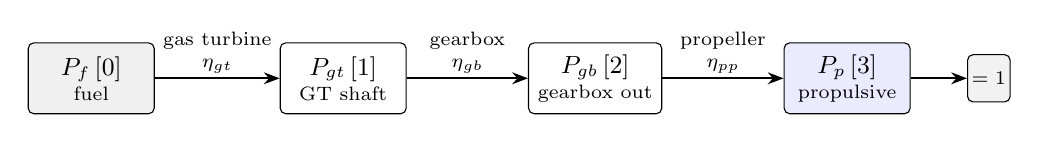
\begin{tikzpicture}[>={Stealth[length=2mm]},
  var/.style={draw, rounded corners=2pt, minimum width=16mm, minimum height=9mm,
              align=center, font=\small, fill=#1}, var/.default=white,
  junction/.style={draw, circle, inner sep=0.5pt, font=\small, fill=white},
  lbl/.style={font=\scriptsize, align=center, inner sep=1.5pt},
  flow/.style={->, thick}, plain/.style={thick},
  splitline/.style={densely dashed, thick, draw=orange!80!black}]
\node[var=gray!12] (Pf) at (0.00,0.00) {$P_{f}$\,[0]\\[-2pt]{\scriptsize fuel}};
\node[var=white] (Pgt) at (3.20,0.00) {$P_{gt}$\,[1]\\[-2pt]{\scriptsize GT shaft}};
\node[var=white] (Pgb) at (6.40,0.00) {$P_{gb}$\,[2]\\[-2pt]{\scriptsize gearbox out}};
\node[var=blue!8] (Pp) at (9.60,0.00) {$P_{p}$\,[3]\\[-2pt]{\scriptsize propulsive}};
\draw[flow] (Pf) -- node[lbl, above] {gas turbine\\$\eta_{gt}$} (Pgt);
\draw[flow] (Pgt) -- node[lbl, above] {gearbox\\$\eta_{gb}$} (Pgb);
\draw[flow] (Pgb) -- node[lbl, above] {propeller\\$\eta_{pp}$} (Pp);
\node[lbl, draw, rounded corners=2pt, fill=gray!10, minimum height=6mm] (sink) at (11.40,0.00) {$=1$};
\draw[flow] (Pp) -- (sink);
\end{tikzpicture}

\caption{\texttt{traditional\_graph}. Generated from the builder.}\label{fig:g-trad}
\end{figure}

\subsection{Turbofan}\label{sec:turbofan}
The \code{'Turbofan'} configuration uses the same builder (Figure~\ref{fig:g-tf}). When
\texttt{Eta Gas Turbine Model} is \code{'Turbofan'}, \code{Powertrain._build_efficiencies}
sets the gas-turbine node to a \code{TurbofanEfficiencyModel} and overrides the gearbox and
propeller nodes with \code{ConstantEfficiency(1.0)}. The first node then carries the overall
efficiency
\begin{equation}
  \eta_o = \frac{F\,V}{\dot m_f\,LHV} ,
\end{equation}
so that $\Pi_0 = 1/\eta_o$ and $\Pi_1 = \Pi_2 = \Pi_3 = 1$. The fuel closure
$P_f = P_p/\eta_o$ is a thrust-specific fuel consumption closure, because
$\mathrm{TSFC} = V/(\eta_o\,LHV)$ (\code{TurbofanEfficiencyModel.tsfc}). The map reads
$\eta_o$ at the thrust $F = P_p/V$, as a fraction of the nominal sea-level-static thrust
\texttt{Turbofan Design Thrust}; the map itself is described in the Engine Decks manual.

The mission and the weight loop reuse \code{TraditionalConfiguration} and
\code{Weight.Traditional} (\code{Mission._fly_configuration}, \code{Weight.WeightEstimation}).
What changes is the sizing quantity: thrust instead of shaft power
(Sections~\ref{sec:lapse} and~\ref{sec:mass-tf}).

\begin{figure}[htbp]
\centering
%% Generated by manuals/powertrain/scripts/make_figures.py from the graph builder.
%% Do not edit by hand.
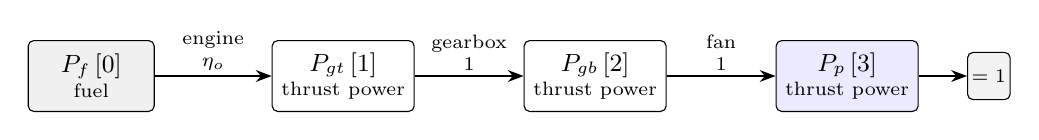
\begin{tikzpicture}[>={Stealth[length=2mm]},
  var/.style={draw, rounded corners=2pt, minimum width=16mm, minimum height=9mm,
              align=center, font=\small, fill=#1}, var/.default=white,
  junction/.style={draw, circle, inner sep=0.5pt, font=\small, fill=white},
  lbl/.style={font=\scriptsize, align=center, inner sep=1.5pt},
  flow/.style={->, thick}, plain/.style={thick},
  splitline/.style={densely dashed, thick, draw=orange!80!black}]
\node[var=gray!12] (Pf) at (0.00,0.00) {$P_{f}$\,[0]\\[-2pt]{\scriptsize fuel}};
\node[var=white] (Pgt) at (3.20,0.00) {$P_{gt}$\,[1]\\[-2pt]{\scriptsize thrust power}};
\node[var=white] (Pgb) at (6.40,0.00) {$P_{gb}$\,[2]\\[-2pt]{\scriptsize thrust power}};
\node[var=blue!8] (Pp) at (9.60,0.00) {$P_{p}$\,[3]\\[-2pt]{\scriptsize thrust power}};
\draw[flow] (Pf) -- node[lbl, above] {engine\\$\eta_o$} (Pgt);
\draw[flow] (Pgt) -- node[lbl, above] {gearbox\\$1$} (Pgb);
\draw[flow] (Pgb) -- node[lbl, above] {fan\\$1$} (Pp);
\node[lbl, draw, rounded corners=2pt, fill=gray!10, minimum height=6mm] (sink) at (11.40,0.00) {$=1$};
\draw[flow] (Pp) -- (sink);
\end{tikzpicture}

\caption{The turbofan: \texttt{traditional\_graph} with the efficiencies that
\texttt{\_build\_efficiencies} assigns for \texttt{'Turbofan'} (checked by the drawing script on the
reference turbofan design).}\label{fig:g-tf}
\end{figure}

\subsection{Parallel hybrid}\label{sec:parallel}
\code{parallel_hybrid_graph(eta_gt, eta_gb, eta_pm, eta_em, eta_pp, phi)} has
the variables $[P_f, P_{gt}, P_{gb}, P_{s1}, P_{e1}, P_{bat}, P_{p1}]$
(Figure~\ref{fig:g-par}). The turbine shaft and the motor shaft enter one gearbox, which is a
combiner:
\begin{equation}
  P_{gt} = \eta_{gt}P_f,\quad
  P_{s1} = \eta_{gb}\,(P_{gt} + P_{gb}),\quad
  P_{e1} = \eta_{pm}P_{bat},\quad
  P_{gb} = \eta_{em}P_{e1},\quad
  P_{p1} = \eta_{pp}P_{s1},
\end{equation}
plus the split~\eqref{eq:phi} and $P_{p1} = 1$. The name $P_{gb}$ denotes the motor shaft
power that enters the gearbox, and $P_{s1}$ the gearbox output. Eliminating the
intermediate powers gives
\begin{equation}
  \Pi_0 = \frac{(1-\varphi)}{\eta_{pp}\eta_{gb}\left[(1-\varphi)\eta_{gt} + \varphi\,\eta_{em}\eta_{pm}\right]},\qquad
  \Pi_5 = \frac{\varphi}{\eta_{pp}\eta_{gb}\left[(1-\varphi)\eta_{gt} + \varphi\,\eta_{em}\eta_{pm}\right]} .
  \label{eq:par}
\end{equation}
The share of $P_p$ delivered by the motor branch is $\eta_{gb}\eta_{pp}\Pi_2$. At
$\varphi = 0$ the graph reduces to the traditional chain.

\begin{figure}[htbp]
\centering
%% Generated by manuals/powertrain/scripts/make_figures.py from the graph builder.
%% Do not edit by hand.
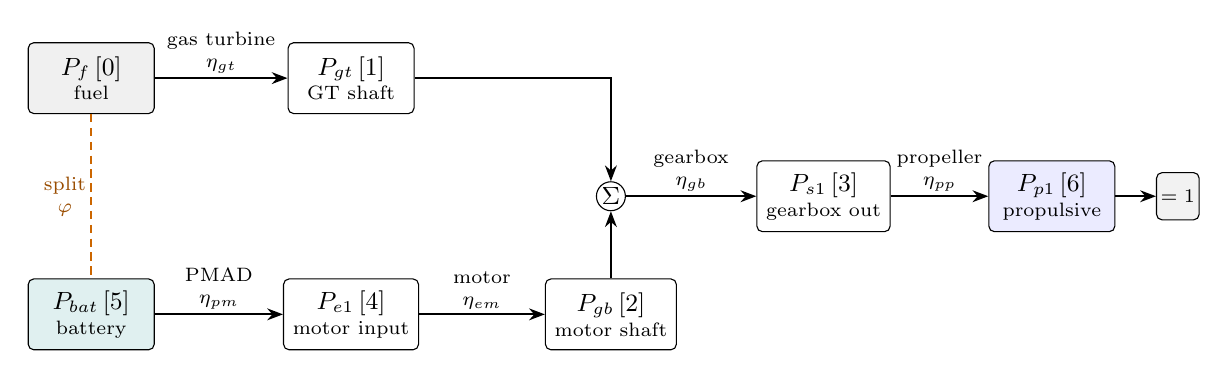
\begin{tikzpicture}[>={Stealth[length=2mm]},
  var/.style={draw, rounded corners=2pt, minimum width=16mm, minimum height=9mm,
              align=center, font=\small, fill=#1}, var/.default=white,
  junction/.style={draw, circle, inner sep=0.5pt, font=\small, fill=white},
  lbl/.style={font=\scriptsize, align=center, inner sep=1.5pt},
  flow/.style={->, thick}, plain/.style={thick},
  splitline/.style={densely dashed, thick, draw=orange!80!black}]
\node[var=gray!12] (Pf) at (0.00,1.50) {$P_{f}$\,[0]\\[-2pt]{\scriptsize fuel}};
\node[var=white] (Pgt) at (3.30,1.50) {$P_{gt}$\,[1]\\[-2pt]{\scriptsize GT shaft}};
\node[var=white] (Pgb) at (6.60,-1.50) {$P_{gb}$\,[2]\\[-2pt]{\scriptsize motor shaft}};
\node[var=white] (Ps1) at (9.30,0.00) {$P_{s1}$\,[3]\\[-2pt]{\scriptsize gearbox out}};
\node[var=white] (Pe1) at (3.30,-1.50) {$P_{e1}$\,[4]\\[-2pt]{\scriptsize motor input}};
\node[var=teal!12] (Pbat) at (0.00,-1.50) {$P_{bat}$\,[5]\\[-2pt]{\scriptsize battery}};
\node[var=blue!8] (Pp1) at (12.20,0.00) {$P_{p1}$\,[6]\\[-2pt]{\scriptsize propulsive}};
\draw[flow] (Pf) -- node[lbl, above] {gas turbine\\$\eta_{gt}$} (Pgt);
\node[junction] (sumPs1) at (6.60,0.00) {$\Sigma$};
\draw[flow] (Pgt) -| (sumPs1);
\draw[flow] (Pgb) -- (sumPs1);
\draw[flow] (sumPs1) -- node[lbl, above] {gearbox\\$\eta_{gb}$} (Ps1);
\draw[flow] (Pbat) -- node[lbl, above] {PMAD\\$\eta_{pm}$} (Pe1);
\draw[flow] (Pe1) -- node[lbl, above] {motor\\$\eta_{em}$} (Pgb);
\draw[flow] (Ps1) -- node[lbl, above] {propeller\\$\eta_{pp}$} (Pp1);
\draw[splitline] (Pf) -- node[lbl, left, text=orange!60!black] {split\\$\varphi$} (Pbat);
\node[lbl, draw, rounded corners=2pt, fill=gray!10, minimum height=6mm] (sink) at (13.80,0.00) {$=1$};
\draw[flow] (Pp1) -- (sink);
\end{tikzpicture}

\caption{\texttt{parallel\_hybrid\_graph}. Generated from the builder.}\label{fig:g-par}
\end{figure}

\subsection{Serial hybrid}\label{sec:serial}
\code{serial_hybrid_graph(eta_gt, eta_em1, eta_pm, eta_em2, eta_gb, eta_pp, phi)}
has the variables
$[P_f, P_{gt}, P_{gb}, P_{s1}, P_{e1}, P_{bat}, P_{gen}, P_{p1}]$ (Figure~\ref{fig:g-ser}).
The turbine drives a generator; the generator output and the battery feed an electrical bus,
which is a combiner with the PMAD efficiency; a motor, a gearbox and the propeller follow:
\begin{equation}
\begin{gathered}
  P_{gt} = \eta_{gt}P_f,\quad
  P_{s1} = \eta_{em1}P_{gt},\quad
  P_{e1} = \eta_{pm}(P_{s1} + P_{bat}),\\
  P_{gb} = \eta_{em2}P_{e1},\quad
  P_{gen} = \eta_{gb}P_{gb},\quad
  P_{p1} = \eta_{pp}P_{gen} .
\end{gathered}
\end{equation}
The variable names follow the legacy solver, and two of them are misleading: $P_{gb}$ is
the motor shaft power and $P_{gen}$ is the \emph{gearbox} output, not the generator output.
The generator output is $P_{s1}$. The solution is
\begin{equation}
  \Pi_0 = \frac{(1-\varphi)}{\eta_{pp}\eta_{gb}\eta_{em2}\eta_{pm}\left[(1-\varphi)\eta_{em1}\eta_{gt} + \varphi\right]},\qquad
  \Pi_5 = \frac{\varphi}{\eta_{pp}\eta_{gb}\eta_{em2}\eta_{pm}\left[(1-\varphi)\eta_{em1}\eta_{gt} + \varphi\right]} .
  \label{eq:ser}
\end{equation}
All the shaft power passes through the electrical chain. At $\varphi = 0$ the serial chain
therefore needs more fuel than the traditional one: $\Pi_0 = 5.7661$ against $5.2609$ with
the reference efficiencies.

\code{Powertrain.Hybrid} passes to this builder the \code{'generator'} entry of
\code{Powertrain.efficiency} as $\eta_{em1}$ and the \code{'electric_motor'} entry as
$\eta_{em2}$. The generator entry is the constant \texttt{Eta Electric Motor 1} unless it is
replaced by hand. The motor entry is the constant \texttt{Eta Electric Motor 2}, the d-q
model when \texttt{Eta Electric Motor Model} is \code{'Smart'}, or the model assigned to
\code{em_model} (Section~\ref{sec:class2}).

\begin{figure}[htbp]
\centering
%% Generated by manuals/powertrain/scripts/make_figures.py from the graph builder.
%% Do not edit by hand.
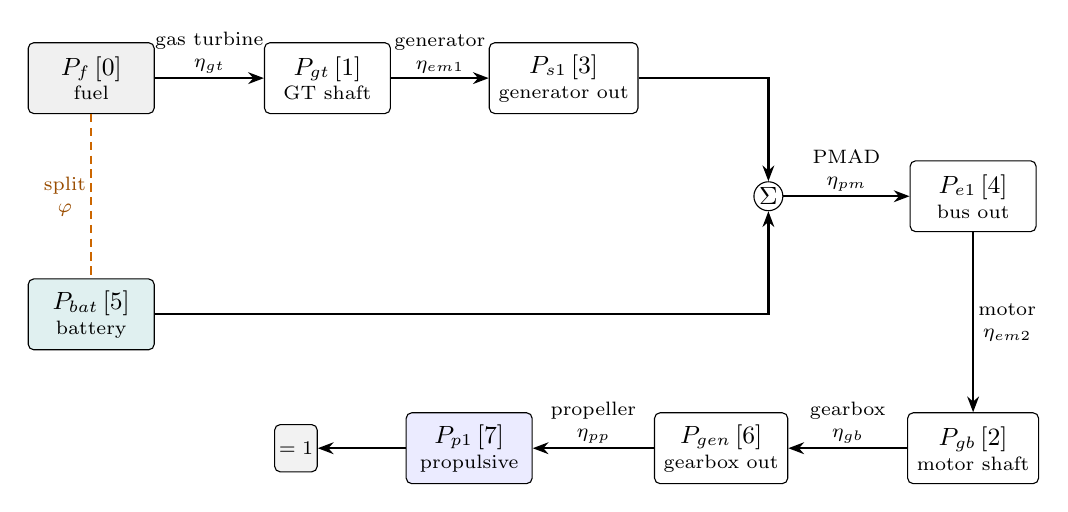
\begin{tikzpicture}[>={Stealth[length=2mm]},
  var/.style={draw, rounded corners=2pt, minimum width=16mm, minimum height=9mm,
              align=center, font=\small, fill=#1}, var/.default=white,
  junction/.style={draw, circle, inner sep=0.5pt, font=\small, fill=white},
  lbl/.style={font=\scriptsize, align=center, inner sep=1.5pt},
  flow/.style={->, thick}, plain/.style={thick},
  splitline/.style={densely dashed, thick, draw=orange!80!black}]
\node[var=gray!12] (Pf) at (0.00,1.50) {$P_{f}$\,[0]\\[-2pt]{\scriptsize fuel}};
\node[var=white] (Pgt) at (3.00,1.50) {$P_{gt}$\,[1]\\[-2pt]{\scriptsize GT shaft}};
\node[var=white] (Pgb) at (11.20,-3.20) {$P_{gb}$\,[2]\\[-2pt]{\scriptsize motor shaft}};
\node[var=white] (Ps1) at (6.00,1.50) {$P_{s1}$\,[3]\\[-2pt]{\scriptsize generator out}};
\node[var=white] (Pe1) at (11.20,0.00) {$P_{e1}$\,[4]\\[-2pt]{\scriptsize bus out}};
\node[var=teal!12] (Pbat) at (0.00,-1.50) {$P_{bat}$\,[5]\\[-2pt]{\scriptsize battery}};
\node[var=white] (Pgen) at (8.00,-3.20) {$P_{gen}$\,[6]\\[-2pt]{\scriptsize gearbox out}};
\node[var=blue!8] (Pp1) at (4.80,-3.20) {$P_{p1}$\,[7]\\[-2pt]{\scriptsize propulsive}};
\draw[flow] (Pf) -- node[lbl, above] {gas turbine\\$\eta_{gt}$} (Pgt);
\draw[flow] (Pgt) -- node[lbl, above] {generator\\$\eta_{em1}$} (Ps1);
\node[junction] (sumPe1) at (8.60,0.00) {$\Sigma$};
\draw[flow] (Ps1) -| (sumPe1);
\draw[flow] (Pbat) -| (sumPe1);
\draw[flow] (sumPe1) -- node[lbl, above] {PMAD\\$\eta_{pm}$} (Pe1);
\draw[flow] (Pe1) -- node[lbl, right] {motor\\$\eta_{em2}$} (Pgb);
\draw[flow] (Pgb) -- node[lbl, above] {gearbox\\$\eta_{gb}$} (Pgen);
\draw[flow] (Pgen) -- node[lbl, above] {propeller\\$\eta_{pp}$} (Pp1);
\draw[splitline] (Pf) -- node[lbl, left, text=orange!60!black] {split\\$\varphi$} (Pbat);
\node[lbl, draw, rounded corners=2pt, fill=gray!10, minimum height=6mm] (sink) at (2.60,-3.20) {$=1$};
\draw[flow] (Pp1) -- (sink);
\end{tikzpicture}

\caption{\texttt{serial\_hybrid\_graph}. Generated from the builder. Note the names: $P_{gb}$
is the motor shaft power and $P_{gen}$ the gearbox output.}\label{fig:g-ser}
\end{figure}

\paragraph{Range extender.} A serial hybrid with the input \texttt{GT Rated Power} is flown by
\code{Mission.SerialRangeExtenderConfiguration} instead. This strategy does not solve the
graph. The turbine runs at its rated power, lapsed with altitude, and
\code{Mission._range_extender_flows} computes the battery power forward along the same chain,
with each efficiency evaluated at the power through its own component:
\begin{equation}
  P_{bat} = \frac{P_p}{\eta_{pp}\,\eta_{gb}\,\eta_{em2}\,\eta_{pm}} - \eta_{em1}P_{gt} .
\end{equation}
$P_{bat}$ is negative when the turbine surplus recharges the battery. The Battery manual
describes this strategy and its sizing.

\subsection{Fuel cell and battery graph}\label{sec:fcb-graph}
\code{fuelcell_battery_graph(eta_fc, eta_pm, eta_em, eta_gb, eta_pp, phi)} has
the variables $[P_{f,\mathrm{H_2}}, P_{fc}, P_{bat}, P_{e1}, P_{em}, P_{gb}, P_{p1}]$
(Figure~\ref{fig:g-fcb}). The fuel cell converts the hydrogen power with $\eta_{fc}$; the
fuel cell and the battery feed a bus, then a motor, a gearbox and the propeller. The split
links the fuel-cell output and the battery, so $\varphi = P_{bat}/(P_{fc} + P_{bat})$ is the
battery share of the propulsive power (Section~\ref{sec:phi}). In this vector the battery is
entry~2, not entry~5. The solution is
\begin{equation}
  \Pi_0 = \frac{1-\varphi}{\eta_{fc}\,\eta_{pm}\,\eta_{em}\,\eta_{gb}\,\eta_{pp}},\qquad
  \Pi_2 = \frac{\varphi}{\eta_{pm}\,\eta_{em}\,\eta_{gb}\,\eta_{pp}} .
  \label{eq:fcb}
\end{equation}

\code{Powertrain.PowerRatioFuelCellBattery} solves this graph with the efficiencies of
\code{Powertrain.eta}. No mission method calls it; Section~\ref{sec:fc-chains} explains why
the missions use their own chains. The graph is still usable. Equation~\eqref{eq:fcb} is the
chain of the mission (Eqs.~\eqref{eq:fc-el} and~\eqref{eq:fcb-bat}) when $\eta_{fc}$ is the
efficiency from hydrogen to the bus and the auxiliary load is folded into it. The graph
therefore gives the hydrogen and battery powers of a split without the stack model, for a
quick estimate, a check of the mission chain, or a teaching example with an assumed
$\eta_{fc}$. It is also the starting point of a new fuel-cell architecture
(Section~\ref{sec:new}). Replacing the split by \code{split("PfH2", "Pbat", phi)} gives the
supplied-power definition of the gas-turbine hybrids, Eq.~\eqref{eq:phi}; the rest of the
graph is unchanged. The fuel-cell efficiency is the constant
\texttt{Eta Fuel Cell} (\code{EnergyConfig.eta_fuel_cell}) or an injected \code{fc_model};
it is not the physics model of the fuel-cell manual. It has no default: without either,
\code{Powertrain.eta('fuel_cell')} raises a \code{ValueError}. \code{Powertrain.SetInput}
reads \texttt{Eta PMAD} and \texttt{Eta Electric Motor} for the two fuel-cell configurations,
so on \code{fuelcell_battery_config()} the powertrain holds $\eta_{pm} = 0.99$ and
$\eta_{em} = 0.96$, the values of the configuration.

\begin{figure}[htbp]
\centering
%% Generated by manuals/powertrain/scripts/make_figures.py from the graph builder.
%% Do not edit by hand.
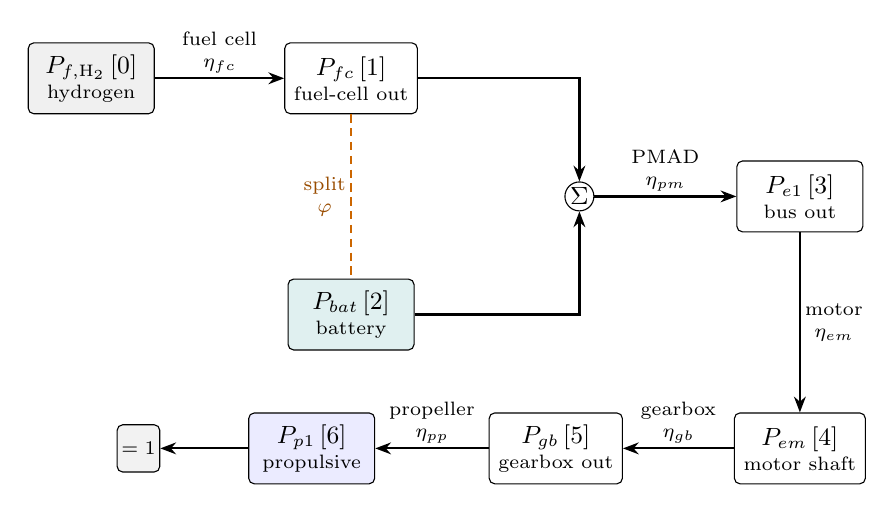
\begin{tikzpicture}[>={Stealth[length=2mm]},
  var/.style={draw, rounded corners=2pt, minimum width=16mm, minimum height=9mm,
              align=center, font=\small, fill=#1}, var/.default=white,
  junction/.style={draw, circle, inner sep=0.5pt, font=\small, fill=white},
  lbl/.style={font=\scriptsize, align=center, inner sep=1.5pt},
  flow/.style={->, thick}, plain/.style={thick},
  splitline/.style={densely dashed, thick, draw=orange!80!black}]
\node[var=gray!12] (PfH2) at (0.00,1.50) {$P_{f,\mathrm{H_2}}$\,[0]\\[-2pt]{\scriptsize hydrogen}};
\node[var=white] (Pfc) at (3.30,1.50) {$P_{fc}$\,[1]\\[-2pt]{\scriptsize fuel-cell out}};
\node[var=teal!12] (Pbat) at (3.30,-1.50) {$P_{bat}$\,[2]\\[-2pt]{\scriptsize battery}};
\node[var=white] (Pe1) at (9.00,0.00) {$P_{e1}$\,[3]\\[-2pt]{\scriptsize bus out}};
\node[var=white] (Pem) at (9.00,-3.20) {$P_{em}$\,[4]\\[-2pt]{\scriptsize motor shaft}};
\node[var=white] (Pgb) at (5.90,-3.20) {$P_{gb}$\,[5]\\[-2pt]{\scriptsize gearbox out}};
\node[var=blue!8] (Pp1) at (2.80,-3.20) {$P_{p1}$\,[6]\\[-2pt]{\scriptsize propulsive}};
\draw[flow] (PfH2) -- node[lbl, above] {fuel cell\\$\eta_{fc}$} (Pfc);
\node[junction] (sumPe1) at (6.20,0.00) {$\Sigma$};
\draw[flow] (Pfc) -| (sumPe1);
\draw[flow] (Pbat) -| (sumPe1);
\draw[flow] (sumPe1) -- node[lbl, above] {PMAD\\$\eta_{pm}$} (Pe1);
\draw[flow] (Pe1) -- node[lbl, right] {motor\\$\eta_{em}$} (Pem);
\draw[flow] (Pem) -- node[lbl, above] {gearbox\\$\eta_{gb}$} (Pgb);
\draw[flow] (Pgb) -- node[lbl, above] {propeller\\$\eta_{pp}$} (Pp1);
\draw[splitline] (Pfc) -- node[lbl, left, text=orange!60!black] {split\\$\varphi$} (Pbat);
\node[lbl, draw, rounded corners=2pt, fill=gray!10, minimum height=6mm] (sink) at (0.60,-3.20) {$=1$};
\draw[flow] (Pp1) -- (sink);
\end{tikzpicture}

\caption{\texttt{fuelcell\_battery\_graph}. Generated from the builder. Not used by the
\texttt{'FuelCellBattery'} mission.}\label{fig:g-fcb}
\end{figure}

\subsection{Fuel-cell chains of the mission}\label{sec:fc-chains}
The \code{'Hydrogen'} and \code{'FuelCellBattery'} missions compute the chain without a
graph (Figure~\ref{fig:fc-chain}). For the fuel-cell share $P_{fc,p}$ of the propulsive
power, \code{FuelCell.ComputePRatio} computes the electrical demand
\begin{equation}
  P_{el} = \frac{P_{fc,p}}{\eta_{gb}\,\eta_{em}\,\eta_{pm}\,\eta_{pp}} + P_{aux,TMS},
  \label{eq:fc-el}
\end{equation}
then solves the stack current for that net power, including the air-system and fixed
auxiliary loads. The hydrogen chemical power is $\dot m_{\mathrm{H_2}}\,HHV$. The
efficiencies are the fuel-cell attributes \code{EtaGB}, \code{EtaEM}, \code{EtaPM} and
\code{EtaProp}, read by \code{FuelCell.SetInput} from the same \code{EnergyInput} keys.
\code{FuelCell.drive_efficiencies} replaces two of them by operating-point models. With the
Hamilton propeller attached, the propeller efficiency is the \code{'propeller'} model of the
powertrain (\code{HamiltonPropellerEfficiency}, bounded to $[0.4, 1]$), evaluated at its
shaft input by a fixed point, damped as in Section~\ref{sec:methods}. When \texttt{Eta Electric Motor Model} is \code{'Smart'}, the
motor efficiency is \code{Powertrain.eta('electric_motor')} at the motor shaft output. In
\code{'FuelCellBattery'} each branch reads these models at its own share of the power, not at
the total power through the shared motor and propeller. The Fuel Cell manual describes the
stack.

In \code{'Hydrogen'}, $P_{fc,p} = P_p$. In \code{'FuelCellBattery'}, $P_{fc,p} =
(1-\varphi)P_p$ and the battery terminal power is
\begin{equation}
  P_{bat} = \frac{\varphi P_p}{\eta_{em}\,\eta_{pm}\,\eta_{gb}\,\eta_{pp}}
  \label{eq:fcb-bat}
\end{equation}
(\code{Mission._fc_battery_terminal_power}). The two branches are computed separately and
share the motor and the PMAD, which are sized on their coincident peak
(Section~\ref{sec:mass-fc}).

The missions use these chains, not the graph of Section~\ref{sec:fcb-graph}, for three
reasons.
\begin{enumerate}
  \item The stack is not a scalar efficiency. \code{FuelCell.ComputePRatio} solves the stack
  current for the net electrical power, including the air-system power, the fixed
  auxiliaries and the TMS pump $P_{aux,TMS}$. These loads add to the demand instead of
  scaling it, so they are not a converter of the graph, whose powers are all proportional
  to $P_p$.
  \item The mission needs the stack state, not only the hydrogen power. Each call stores the
  operating current and voltage, the heat to the TMS (with the product-water vapour
  fraction), the power-limited flag and the effect of the state of health. The TMS sizing,
  the off-design checks and the degradation studies read them.
  \item With $\varphi$ a share of the propulsive power, the fuel-cell load $(1-\varphi)P_p$
  is known before the stack is solved, so every mission point is explicit. With the
  supplied-power definition, Eq.~\eqref{eq:phi}, the hydrogen power depends on the stack
  efficiency at its own load, and the split at each point would need an iteration through
  the polarization curve. The propulsive share also maps directly onto the stack rating: on a
  field where the take-off sizes the fuel cell, the battery that brings the take-off load
  down to the climb load is $\varphi^* = 1 - P_{climb}/P_{TO}$ (example 23).
\end{enumerate}

\begin{figure}[htbp]
\centering
\begin{tikzpicture}[>={Stealth[length=2mm]},
  var/.style={draw, rounded corners=2pt, minimum width=16mm, minimum height=9mm,
              align=center, font=\small, fill=#1}, var/.default=white,
  lbl/.style={font=\scriptsize, align=center, inner sep=1.5pt},
  flow/.style={->, thick}]
  \node[var=gray!12] (h2) at (0,1.4) {H$_2$\\[-2pt]{\scriptsize $\dot m_{\mathrm{H_2}}HHV$}};
  \node[var] (pel) at (4.8,1.4) {$P_{el}$\\[-2pt]{\scriptsize net electric}};
  \node[var] (fcp) at (9.6,1.4) {$(1-\varphi)P_p$\\[-2pt]{\scriptsize fuel-cell share}};
  \node[var=teal!12] (bat) at (0,-1.4) {$P_{bat}$\\[-2pt]{\scriptsize battery terminal}};
  \node[var] (bp) at (9.6,-1.4) {$\varphi P_p$\\[-2pt]{\scriptsize battery share}};
  \node[var=blue!8] (pp) at (12.6,0) {$P_p$\\[-2pt]{\scriptsize propulsive}};
  \draw[flow] (h2) -- node[lbl, above] {stack + air system\\\code{ComputePRatio}} (pel);
  \draw[flow] (pel) -- node[lbl, above] {$\eta_{pm}\,\eta_{em}\,\eta_{gb}\,\eta_{pp}$\\(minus $P_{aux,TMS}$)} (fcp);
  \draw[flow] (bat) -- node[lbl, above] {$\eta_{em}\,\eta_{pm}\,\eta_{gb}\,\eta_{pp}$\\\code{_fc_battery_eta_elec}} (bp);
  \draw[flow] (fcp) -| (pp);
  \draw[flow] (bp) -| (pp);
\end{tikzpicture}
\caption{Chains of the fuel-cell missions, drawn by hand from \texttt{FuelCell.ComputePRatio}
and \texttt{Mission.\_fc\_battery\_eta\_elec} (not a \texttt{PowertrainGraph}). In
\texttt{'Hydrogen'} the battery branch is absent and $\varphi = 0$.}\label{fig:fc-chain}
\end{figure}

\subsection{Index reference}\label{sec:indices}
Table~\ref{tab:indices} lists the power-ratio vectors returned by the \code{Powertrain}
methods and the entries that other modules read. The entries 0, 1, 2, 4 and 5 of
\code{Hybrid} have the same meaning in the parallel and serial vectors: fuel, turbine shaft,
motor shaft, motor input and battery.

\begin{table}[htbp]
\centering\small
\caption{Power-ratio vectors (all divided by $P_p$) and their consumers.}\label{tab:indices}
\begin{tabularx}{\textwidth}{@{}lX@{}}
\toprule
Method & Vector and consumers \\
\midrule
\code{Traditional} & $[P_f, P_{gt}, P_{gb}, P_p]$. [0] fuel energy rate (\code{TraditionalConfiguration}, \code{_ground_power_split}, \code{ClimateImpact}); [1] shaft power for \code{Max_PEng} and \code{TO_PP}. \\
\code{Hybrid} (parallel) & $[P_f, P_{gt}, P_{gb}, P_{s1}, P_{e1}, P_{bat}, P_{p1}]$. [0] fuel; [1] turbine shaft (\code{Max_PEng}, \code{TO_PP}); [2] motor shaft (\code{Max_PMotor}, \code{TO_PMotor}); [4] motor input (\code{Max_PBus}, \code{TO_PBus}); [5] battery terminal power (battery energy, \code{Max_PBat}, \code{TO_PBat}, Class-II pack current). \\
\code{Hybrid} (serial) & $[P_f, P_{gt}, P_{gb}, P_{s1}, P_{e1}, P_{bat}, P_{gen}, P_{p1}]$. Same consumers as parallel; [4] is the bus output into the motor. \\
\code{PowerRatioFuelCellBattery} & $[P_{f,\mathrm{H_2}}, P_{fc}, P_{bat}, P_{e1}, P_{em}, P_{gb}, P_{p1}]$. No consumer in the mission. \\
\bottomrule
\end{tabularx}
\end{table}

%% ======================================================================================
\section{The Powertrain class}\label{sec:class}
%% ======================================================================================

\subsection{Inputs}
\code{Powertrain.SetInput} reads \code{aircraft.EnergyInput}. The keys it needs
depend on the configuration:
\begin{itemize}
\item every configuration except \code{'Turbofan'} needs \texttt{Eta Gearbox} and
  \texttt{Specific Power Powertrain}, a list [thermal, electric motor] in W/kg; a turbofan
  defaults them to 1.0 and [0, 0];
\item \code{'Hybrid'} needs \texttt{Eta PMAD}; \code{'Parallel'} also needs
  \texttt{Eta Electric Motor}, and \code{'Serial'} needs \texttt{Eta Electric Motor 1} (the
  generator) and \texttt{Eta Electric Motor 2} (the motor);
\item \code{'Hydrogen'} and \code{'FuelCellBattery'} need \texttt{Eta PMAD} and
  \texttt{Eta Electric Motor};
\item \texttt{Eta Gas Turbine} and \texttt{Eta Propulsive} are read when present. When one is
  absent and its model is constant, \code{SetInput} issues a \code{UserWarning} and the
  constant model of \code{_build_efficiencies} uses 0.30 or 0.85; the configurations without
  a gas turbine or a propeller of that kind skip the warning;
\item the number of engines is \texttt{PropellerInput['Number of Engines']}, default 2
  (\code{Powertrain.n_engines}); the Class-II maps, the Hamilton propeller and the emission
  model divide the total power by it;
\item \texttt{Specific Power PMAD}, \texttt{Specific Power Generator} and \texttt{Eta Fuel Cell}
  are optional.
\end{itemize}
The remaining inputs select the Class-II models (Section~\ref{sec:class2}).
Table~\ref{tab:inputs} lists all of them.

\subsection{Component efficiencies}
\code{_build_efficiencies} stores one \code{EfficiencyModel} per component in the
dictionary \code{Powertrain.efficiency}, with the keys \code{'gas_turbine'},
\code{'gearbox'}, \code{'pmad'}, \code{'electric_motor'}, \code{'propeller'} and
\code{'generator'}. The \code{'electric_motor'} entry is \texttt{Eta Electric Motor 2} in a
serial hybrid and \texttt{Eta Electric Motor} otherwise; the \code{'generator'} entry is
\texttt{Eta Electric Motor 1}, or 1.0 in the architectures without a generator. The fuel cell
has no entry: \code{eta} reads \code{fc_model} or \texttt{Eta Fuel Cell}. Each entry is a \code{ConstantEfficiency} unless the configuration
selects a Class-II model: \texttt{Eta Gas Turbine Model} = \code{'ResponseSurface'} or
\code{'Turbofan'}, \texttt{Eta Propulsive Model} = \code{'Hamilton'}, \code{'Surrogate'} or
\code{'RBF'}, and \texttt{Eta Electric Motor Model} = \code{'Smart'}. The turbofan and the
motor need a nominal rating fixed before the mission (\texttt{Turbofan Design Thrust},
\texttt{EM Design Power}); the method raises a \code{ValueError} without it. The Class-II gas
turbine takes \texttt{GT Design Power} as a fixed nominal when it is given. Without it, the
nominal follows the sized \code{engineRating} in the weight loop
(\code{Weight._mission_and_powertrain}).

\code{Powertrain.eta(component, alt, vel, pwr, rpm)} builds an
\code{OperatingPoint} and evaluates the model of that component. Two attributes,
\code{em_model} and \code{fc_model}, override the electric-motor and fuel-cell entries when
they are set; both default to \code{None}.

\subsection{Power-ratio methods}\label{sec:methods}
Three methods assemble a graph at the current operating point and solve it:
\begin{itemize}
\item \code{Traditional(alt, vel, pwr)} returns the solution of
  \code{traditional_graph};
\item \code{Hybrid(phi, alt, vel, pwr)} stores \code{self.phi} and returns
  \code{numpy.abs} of \code{parallel_hybrid_graph} or \code{serial_hybrid_graph}, according
  to \code{aircraft.HybridType}; it raises for any other value;
\item \code{PowerRatioFuelCellBattery(phi, alt, vel, pwr)} returns \code{numpy.abs}
  of \code{fuelcell_battery_graph}.
\end{itemize}
A new graph is built at every call, and at every pass of the fixed point described below. Its
cost is negligible next to the mission integration.

The power argument \code{pwr} that the mission passes is the propulsive power $P_p$ of the
whole aircraft. Each efficiency model is evaluated at the power through its own component,
all engines together, in the convention of Table~\ref{tab:convention}. These powers depend on
the efficiencies, so \code{_solve_at_component_powers} finds them by a fixed point. The
first pass evaluates every model at $P_p$ and solves the graph. Each further pass
re-evaluates the models at updated component powers, until the powers the models were read
at match the solved powers within $10^{-6}\,|P_p|$ (\code{COMPONENT_POWER_RTOL}), with at
most 50 passes and a warning when they do not converge. The iteration is damped: each pass
moves the powers by a fraction \code{relax} of the step towards the solved powers. The
fraction starts at 1 and is halved whenever the step of any operating-point dependent
component changes sign. The docstring gives the reason: the efficiency of a propeller at low
power rises steeply with its shaft power, and the undamped iteration overshoots and
oscillates around the solution. When every model of the graph is a
\code{ConstantEfficiency}, the first solution is returned as it is, so constant-efficiency
results do not depend on this iteration. On the traditional reference chain the gas-turbine
shaft carries $\Pi_1 = 1.1574$ times $P_p$, and on the parallel chain at $\varphi = 0.3$ the
motor shaft carries $\Pi_2 = 0.7569$ times $P_p$.

\begin{table}[htbp]
\centering\small
\caption{Power at which \texttt{Powertrain.eta} evaluates each component model (docstring of
\texttt{eta}).}\label{tab:convention}
\begin{tabularx}{\textwidth}{@{}lX@{}}
\toprule
Component & Power passed to the model \\
\midrule
\code{gas_turbine} & shaft output ($P_p\Pi_1$) \\
\code{propeller} & shaft input \\
\code{electric_motor} & shaft output ($P_p\Pi_2$ in the hybrids) \\
\code{generator} & electrical output (serial hybrid, $P_p\Pi_3$) \\
\code{gearbox} & input (sum of the two shafts in the parallel hybrid) \\
\code{pmad} & input (sum of the sources it combines) \\
\code{fuel_cell} & net electrical output \\
\bottomrule
\end{tabularx}
\end{table}

\subsection{Legacy solvers and equivalence}\label{sec:legacy}
\code{_traditional_legacy} and \code{_hybrid_legacy} keep the
hand-written $4\times4$, $7\times7$ and $8\times8$ matrices from which the builders were
derived. They are kept only as references for the equivalence tests and are not called by
the model. \code{tests/regression/test_powertrain_equivalence.py} sweeps three altitudes,
three speeds, two powers and four values of $\varphi$, and asserts that the graph methods
return the same vectors. Our script repeats the sweep with five values of $\varphi$ (0, 0.1,
0.3, 0.5, 0.8) on the reference configurations. Over 18 traditional points and 90 points
for each hybrid type, the largest absolute difference is 0.0: the two solvers agree to the
last bit. The legacy solvers evaluate the models at $P_p$, and the legacy serial solver
uses the attribute \code{EtaGT} directly, so the equivalence holds for constant efficiencies
only. \code{tests/regression/test_powertrain_component_powers.py} checks the component powers
of the graph methods and that constant models give the plain graph solution bit for bit. The golden-master tests
(\code{tests/regression/test_golden_design.py}) pin the full traditional and parallel-hybrid
designs.

%% ======================================================================================
\section{Class-II efficiency models}\label{sec:class2}
%% ======================================================================================

\subsection{The interface}
\code{efficiency.py} defines an \code{OperatingPoint} with the fields \code{altitude} [m],
\code{velocity} (true airspeed) [m/s], \code{power} [W], and the optional \code{rpm},
\code{voltage} and a dictionary \code{extras}. An \code{EfficiencyModel} has one abstract
method, \code{eta(op)}, which returns an efficiency in $(0, 1]$. Any object that implements
it can stand in a graph node, through \code{Powertrain.efficiency} or the overrides
\code{em_model} and \code{fc_model}.

\subsection{Generic models}
Three generic models cover most needs:
\begin{itemize}
\item \code{ConstantEfficiency(value)} returns \code{value} at any point. It is the default
  of every component.
\item \code{CallableEfficiency(fn)} returns \code{float(fn(op))}. It wraps an analytic law or
  a call to an external code.
\item \code{ResponseSurfaceEfficiency(predictor, features, clip=(0, 1))} wraps a fitted
  surrogate. \code{features} is a list of \code{OperatingPoint} attribute names or a function
  of \code{op}; \code{predictor} is an object with \code{predict} or a plain function. The
  prediction is clipped to \code{clip}. \code{from_file(path, features)} loads the predictor
  with \code{joblib}, then with \code{pickle}.
\end{itemize}
\code{make_efficiency_model(spec)} builds a model from a compact specification: an
\code{EfficiencyModel} is returned unchanged, a number gives a constant, a callable gives a
\code{CallableEfficiency}, and a dictionary with \code{'type'} = \code{'constant'} or
\code{'response_surface'} gives the corresponding model. Any other input raises.

\subsection{The d-q electric motor}\label{sec:motor}
\code{MotorEfficiencyModel(design_kw, design_v, design_rpm, n_engines)} wraps
\code{EM.ElectricMotor}. The motor is scaled from a reference machine of \SI{750}{kW},
\SI{800}{V} and \SI{3000}{rpm} (\code{_generate_scaled_params}). At an operating point,
\code{MotorEfficiencyModel.eta} divides the power by the number of engines, converts it to a
torque at the operating rpm (the design rpm when \code{op.rpm} is \code{None}), and calls
\code{solve_efficiency}. That method computes the $q$-axis current from the torque plus
friction, applies field weakening when the back-electromotive force exceeds the voltage
limit, and returns
\begin{equation}
  \eta_{em} = \frac{P_{out}}{P_{out} + P_{cu} + P_{core} + P_{wind} + P_{const}},
\end{equation}
with copper, core, windage and constant losses. It returns 0.05 for an infeasible point, and
\code{MotorEfficiencyModel} floors the result at 0.05. The constants of the reference machine
and the loss laws have no source in the code. \code{MotorEfficiencyModel.weight} estimates
the mass of one motor; the sizing does not use it.

The model is selected in two ways. With \texttt{Eta Electric Motor Model} = \code{'Smart'}, it
replaces the motor entry of \code{Powertrain.efficiency}, scaled by \texttt{EM Design Power},
\texttt{EM Design Voltage} (default \SI{800}{V}) and \texttt{EM Design RPM} (default
\SI{11000}{rpm}). Alternatively, any instance can be assigned to \code{em_model}.
Section~\ref{sec:res-motor} shows its effect.

\subsection{Engine decks}
The other Class-II models wrap response surfaces of engines and propellers:
\code{GasTurbineEfficiencyModel} (turboshaft map read at the shaft power as a fraction of
the nominal power), \code{TurbofanEfficiencyModel} (Section~\ref{sec:turbofan}),
\code{HamiltonPropellerEfficiency} (Hamilton-Standard method, clipped to $[0.4, 1]$) and
\code{PropellerSurrogateEfficiency} (RBF surrogate with a pitch governor at \code{Propeller
RPM}, default 1200). Their data, fits and validity are the subject of the Engine Decks
manual.

\subsection{Nominal-rating checks}\label{sec:checks}
A Class-II engine or motor is read at a fraction of a nominal rating chosen before the
mission. Two methods check that choice after the design.
\code{report_class_ii_sizing(raise_on_undersize=False)} walks the mission
(\code{_thermal_power_timeline}), compares the gas-turbine shaft power $P_p\Pi_1$ with the
power available from the map at each point, and compares the peak motor shaft power
(the larger of \code{Max_PMotor} and \code{TO_PMotor}) with \texttt{EM Design Power}. The gas-turbine
check runs when \texttt{GT Design Power} is given. It reports \code{UNDERSIZED} above a load ratio of 1,
\code{oversized} below 0.5, and warns or raises. \code{report_turbofan_sizing(warn=True)}
reports which of the three thrust cases of Section~\ref{sec:mass-tf} sizes the engine and
compares it with \texttt{Turbofan Design Thrust}, with the same two thresholds. Example
\code{16_class_ii_propulsion_sizing.py} shows the workflow.

%% ======================================================================================
\section{Powertrain rating and mass}\label{sec:mass}
%% ======================================================================================

\code{Powertrain.WeightPowertrain(WTO)} returns the powertrain mass
\code{Weight.WPT} of the three configurations that use a gas turbine or a turbofan. The
fuel-cell configurations size their electric drive inside the fuel-cell model
(Section~\ref{sec:mass-fc}). All component masses are a rated power divided by a constant
specific power.

\subsection{Power lapse and the sizing denominator}\label{sec:lapse}
\code{PowerLapse(altitude, DISA)} is the full-throttle power lapse. With a
constant gas-turbine efficiency it is
\begin{equation}
  \lambda(h) = \left(\frac{\rho(h)}{\rho(0)}\right)^{0.75},
\end{equation}
from Ruijgrok~\cite{ruijgrok}, Eq.~(6.7-11), as cited in the docstring. With the Class-II
gas-turbine map (\code{gas_turbine_has_map_lapse}) it is the lapse of the map itself, the ISA
pressure ratio $\delta(h)$ of \code{gas_turbine_surrogate._isa_pressure_ratio}, without Mach or
\code{DISA} dependence, so the engine is rated with the full power it has on the map. The
constraint diagram divides each required power-to-weight by
\code{SizingDenominator(altitude, DISA)}. For every power-rated configuration this is $\lambda(h)$, or 1 when the altitude
lapse is switched off. For \code{'Turbofan'} it is $g\,V\,\alpha(h, M)$, with the thrust
lapse \code{ThrustLapse} taken from the fitted map or, without a map, from the form
$\delta\,(1 - 0.49\sqrt{M})$ that the docstring attributes to Mattingly. The design point of
a turbofan is therefore a dimensionless thrust-to-weight ratio.
\code{tests/regression/test_sizing_denominator.py} checks that the denominator equals the
power lapse for the power-rated configurations.

\subsection{Traditional}
The engine rating is the larger of the mission peak shaft power referred to sea level and the
shaft power at the take-off/one-engine-inoperative (OEI) worst case:
\begin{equation}
  P_{rating} = \max\left(\frac{P_{gt,max}}{\lambda(h_{max})},\; P_{gt,TO}\right),\qquad
  W_{thermal} = \frac{P_{rating}}{p_{th}} ,
  \label{eq:rating}
\end{equation}
with $P_{gt,max}$ = \code{mission.Max_PEng} at altitude \code{Max_PEng_alt},
$P_{gt,TO}$ = \code{mission.TO_PP} (the shaft power at the worse of take-off and OEI climb,
\code{Mission._worst_case_propulsive_power}) and $p_{th}$ the first entry of
\texttt{Specific Power Powertrain}. The lapse is evaluated with \code{DISA} = 0. The rating is
stored as \code{engineRating} and the mass as \code{WThermal}. With the Class-II map,
\code{_map_lapse_engine_rating} takes instead the largest $P_{gt}/\delta(h)$ over all mission
points (\code{Max_PEng_lapsed}) and $P_{gt,TO}/\delta(h_{TO})$, so the map covers every
point of the mission.

\subsection{Hybrid}
The thermal part follows Eq.~\eqref{eq:rating} with the turbine shaft power $P_p\Pi_1$. The
electric drive depends on the topology. In the parallel hybrid the motor and the PMAD carry
only the battery power:
\begin{equation}
  W_{motor} = \frac{\max(P_{bat,max}, P_{bat,TO})}{p_{em}},\qquad
  W_{PMAD} = \frac{\max(P_{bat,max}, P_{bat,TO})}{p_{PMAD}} .
\end{equation}
In the serial hybrid the motor carries the whole shaft power to the propeller, the generator
the whole turbine rating, and the PMAD the whole bus power:
\begin{equation}
  W_{motor} = \frac{\max(P_{mot,max}, P_{mot,TO})}{p_{em}} + \frac{P_{rating}}{p_{gen}},\qquad
  W_{PMAD} = \frac{\max(P_{bus,max}, P_{bus,TO})}{p_{PMAD}} ,
\end{equation}
where $P_{mot} = P_p\Pi_2$ and $P_{bus} = P_p\Pi_4$ are tracked by the mission
(\code{Max_PMotor}, \code{TO_PMotor}, \code{Max_PBus}, \code{TO_PBus}). Here $p_{em}$ is the
second entry of \texttt{Specific Power Powertrain}, $p_{gen}$ is \texttt{Specific Power Generator}
(default $p_{em}$) and $p_{PMAD}$ is \texttt{Specific Power PMAD}. The code returns
\SI{10000}{W/kg} for an absent PMAD value (\code{pmad_specific_power}); its docstring calls
this value current to near-term power electronics without a source. The generator mass is
stored as \code{WGenerator} and included in \code{WMotor}; \code{WElectric} is
\texttt{WMotor + WPMAD}. Before the sizing, \code{Mission.EvaluateMission} raises
\code{Max_PBat} to the take-off-run and taxi battery powers of the ground segments (Battery
manual).

\subsection{Turbofan}\label{sec:mass-tf}
A turbofan is rated on sea-level-static thrust. \code{WeightPowertrain} takes the largest of
three requirements, each referred to sea level by the thrust lapse:
\begin{equation}
\begin{gathered}
  T_{rating} = \max\left(\frac{T_{max}}{\alpha(h_{max}, M_{max})},\;
  \frac{T_{TO}}{\alpha(h_{TO}, M_{TO})},\; \left(\frac{T}{W}\right)_{design} W_{TO}\,g\right),\\
  W_{thermal} = \frac{T_{rating}}{g\,(T/W)_{eng}} .
\end{gathered}
\end{equation}
The first term is the mission point with the largest thrust-to-lapse ratio
(\code{TraditionalConfiguration}), the second the take-off/OEI thrust, the third the
constraint diagram. $(T/W)_{eng}$ is \texttt{Engine Thrust to Weight}, default 5.5, described
in the code as CFM56 class without a source. \code{engineRating} then holds a thrust in
newtons, and \code{results().engineRating_units} is \code{'N'}.

\subsection{Fuel-cell configurations}\label{sec:mass-fc}
In \code{'Hydrogen'} and \code{'FuelCellBattery'}, \code{Weight.WPT} is the fuel-cell system
mass \code{FuelCell.Weight}. \code{FuelCell._size_stack} adds to the stack and the balance
of plant a motor and a PMAD sized with the same specific powers as the hybrid powertrain:
\begin{equation}
  P_{drive,el} = \frac{P_{drive}}{\eta_{em}\eta_{pm}\eta_{gb}\eta_{pp}},\qquad
  W_{motor} = \frac{P_{drive,el}\,\eta_{pm}}{p_{em}},\qquad
  W_{PMAD} = \frac{P_{drive,el} + P_{aux,TMS}}{p_{PMAD}} .
\end{equation}
In \code{'Hydrogen'}, $P_{drive}$ is the propulsive power the stack is sized for. In
\code{'FuelCellBattery'} the battery feeds the same PMAD and motor, so $P_{drive}$ is the
larger of that power and \code{mission.Max_PDrive}, the peak propulsive power through the
drive at one instant (fuel-cell and battery shares together, over the mission, the
take-off/OEI point and the ground legs), times \code{SizingMargin}. A design with
$\varphi = 0$ therefore keeps the drive of the \code{'Hydrogen'} design. The Fuel Cell manual
describes the stack mass.

\subsection{Double counting}
Class-I structural regressions are empty-weight fractions, so they already contain the
engines. \code{Weight.powertrain_in_closure} returns 0 instead of \code{WPT} when
\code{avoid_powertrain_double_count} is set and the structural model contains the powertrain.
\code{turbofan_config()} sets it; the other reference configurations do not. \code{WPT} is
still computed and reported.

%% ======================================================================================
\section{Adding a new architecture}\label{sec:new}
%% ======================================================================================

A new architecture is a new composition of the primitives. As a worked example we build a
partial turbo-electric powertrain. One gas turbine drives a gearbox and a main propeller,
and also a generator. The generator feeds a PMAD and a motor that drives an electric fan. The
fan produces the share $\xi$ of the total propulsive power. The script
\code{manuals/powertrain/scripts/example_new_architecture.py} is listed below and runs as
it is:

\lstinputlisting{scripts/example_new_architecture.py}

Three features of the example generalize. First, a lossless junction is a combiner with
efficiency 1: \code{combiner("Pgt", ["Pa", "Pb"], 1.0)} states $P_{gt} = P_a + P_b$, and
\code{combiner("Pp", ["Pp1", "Pp2"], 1.0)} adds the thrust powers of the two propulsors.
Second, the split can link any two variables: here it fixes the share of the fan in the
propulsive power, $\xi = P_{p2}/(P_{p1} + P_{p2})$, and not a share of the supplied power.
Third, the system must stay square: 11 variables need 11 equations. Figure~\ref{fig:g-new} is
generated from this builder by the same script as the other drawings.

\begin{figure}[htbp]
\centering
%% Generated by manuals/powertrain/scripts/make_figures.py from the graph builder.
%% Do not edit by hand.
\resizebox{\linewidth}{!}{%
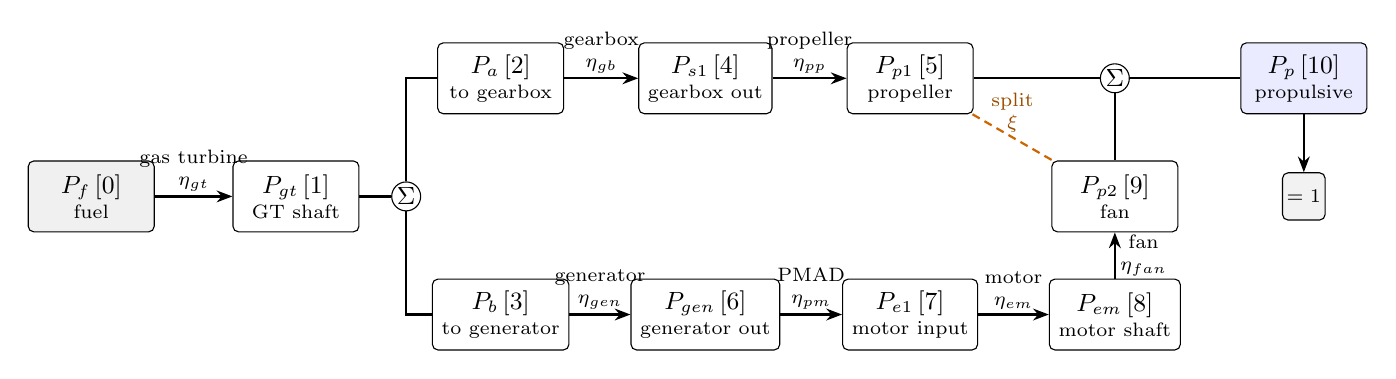
\begin{tikzpicture}[>={Stealth[length=2mm]},
  var/.style={draw, rounded corners=2pt, minimum width=16mm, minimum height=9mm,
              align=center, font=\small, fill=#1}, var/.default=white,
  junction/.style={draw, circle, inner sep=0.5pt, font=\small, fill=white},
  lbl/.style={font=\scriptsize, align=center, inner sep=1.5pt},
  flow/.style={->, thick}, plain/.style={thick},
  splitline/.style={densely dashed, thick, draw=orange!80!black}]
\node[var=gray!12] (Pf) at (0.00,0.00) {$P_{f}$\,[0]\\[-2pt]{\scriptsize fuel}};
\node[var=white] (Pgt) at (2.60,0.00) {$P_{gt}$\,[1]\\[-2pt]{\scriptsize GT shaft}};
\node[var=white] (Pa) at (5.20,1.50) {$P_{a}$\,[2]\\[-2pt]{\scriptsize to gearbox}};
\node[var=white] (Pb) at (5.20,-1.50) {$P_{b}$\,[3]\\[-2pt]{\scriptsize to generator}};
\node[var=white] (Ps1) at (7.80,1.50) {$P_{s1}$\,[4]\\[-2pt]{\scriptsize gearbox out}};
\node[var=white] (Pp1) at (10.40,1.50) {$P_{p1}$\,[5]\\[-2pt]{\scriptsize propeller}};
\node[var=white] (Pgen) at (7.80,-1.50) {$P_{gen}$\,[6]\\[-2pt]{\scriptsize generator out}};
\node[var=white] (Pe1) at (10.40,-1.50) {$P_{e1}$\,[7]\\[-2pt]{\scriptsize motor input}};
\node[var=white] (Pem) at (13.00,-1.50) {$P_{em}$\,[8]\\[-2pt]{\scriptsize motor shaft}};
\node[var=white] (Pp2) at (13.00,0.00) {$P_{p2}$\,[9]\\[-2pt]{\scriptsize fan}};
\node[var=blue!8] (Pp) at (15.40,1.50) {$P_{p}$\,[10]\\[-2pt]{\scriptsize propulsive}};
\draw[flow] (Pf) -- node[lbl, above] {gas turbine\\$\eta_{gt}$} (Pgt);
\node[junction] (sumPgt) at (4.00,0.00) {$\Sigma$};
\draw[plain] (Pa) -| (sumPgt);
\draw[plain] (Pb) -| (sumPgt);
\draw[plain] (sumPgt) -- (Pgt);
\draw[flow] (Pa) -- node[lbl, above] {gearbox\\$\eta_{gb}$} (Ps1);
\draw[flow] (Ps1) -- node[lbl, above] {propeller\\$\eta_{pp}$} (Pp1);
\draw[flow] (Pb) -- node[lbl, above] {generator\\$\eta_{gen}$} (Pgen);
\draw[flow] (Pgen) -- node[lbl, above] {PMAD\\$\eta_{pm}$} (Pe1);
\draw[flow] (Pe1) -- node[lbl, above] {motor\\$\eta_{em}$} (Pem);
\draw[flow] (Pem) -- node[lbl, right] {fan\\$\eta_{fan}$} (Pp2);
\node[junction] (sumPp) at (13.00,1.50) {$\Sigma$};
\draw[plain] (Pp1) -- (sumPp);
\draw[plain] (Pp2) -- (sumPp);
\draw[plain] (sumPp) -- (Pp);
\draw[splitline] (Pp1) -- node[lbl, above, text=orange!60!black] {split\\$\xi$} (Pp2);
\node[lbl, draw, rounded corners=2pt, fill=gray!10, minimum height=6mm] (sink) at (15.40,0.00) {$=1$};
\draw[flow] (Pp) -- (sink);
\end{tikzpicture}%
}

\caption{The partial turbo-electric example. Generated from
\texttt{partial\_turboelectric\_graph}. The junctions with efficiency 1 are drawn without
arrows.}\label{fig:g-new}
\end{figure}

With the efficiencies of \code{common.py} and $\eta_{fan} = \eta_{pp}$, the script prints:
\begin{center}\small
\begin{tabular}{@{}cccc@{}}
\toprule
$\xi$ & $P_f/P_p$ (graph) & $P_f/P_p$ (closed form) & generator input $P_b/P_p$ \\
\midrule
0.0 & 5.2609 & 5.2609 & 0.0000 \\
0.2 & 5.3159 & 5.3159 & 0.2436 \\
0.5 & 5.3982 & 5.3982 & 0.6089 \\
\bottomrule
\end{tabular}
\end{center}
The graph matches the closed form. At $\xi = 0$ the architecture reduces to the traditional
chain, with the same $P_f/P_p$ as Eq.~\eqref{eq:trad}.

\paragraph{From a graph to a design.} The graph gives the power balance only. To fly and size
an aircraft with it, three more pieces are needed, as for the existing architectures. First,
a \code{Powertrain} method that evaluates the efficiencies with \code{self.eta} and returns
the solution vector. Second, a \code{Mission.*Configuration} method that integrates the
energy rates from the entries it needs and records the peak powers for the sizing. Third, a
branch of \code{WeightPowertrain} and of \code{Weight.WeightEstimation}, selected by a new
value of \code{Configuration}, which \code{AircraftConfig.__post_init__} must also accept.
The developer guide \code{docs/developer-guide/extending-the-model.md} lists the same steps.

%% ======================================================================================
\section{Results on the reference designs}\label{sec:results}
%% ======================================================================================

\subsection{Power ratios at the reference efficiencies}\label{sec:res-ratios}
Table~\ref{tab:ratios} gives the solution vectors of the four graphs at $\varphi = 0$ and
$\varphi = 0.3$. The gas-turbine graphs use the efficiencies of \code{hybrid_config}. The
fuel-cell graph uses $\eta_{fc} = 0.5$, an illustrative constant set by the script (the code
has no default), and the electric efficiencies
of \code{fuelcell_battery_config} ($\eta_{pm} = 0.99$, $\eta_{em} = 0.96$,
$\eta_{gb} = 0.96$, $\eta_{pp} = 0.85$). The methods \code{Traditional}, \code{Hybrid} and
\code{PowerRatioFuelCellBattery} of the configured powertrains return the same vectors.

\begin{table}[htbp]
\centering\small
\caption{Power-ratio vectors $\Pi_k$ of the reference chains.}\label{tab:ratios}
\setlength{\tabcolsep}{4pt}
\begin{tabular}{@{}lccccccccc@{}}
\toprule
Graph & $\varphi$ & $\Pi_0$ & $\Pi_1$ & $\Pi_2$ & $\Pi_3$ & $\Pi_4$ & $\Pi_5$ & $\Pi_6$ & $\Pi_7$ \\
\midrule
traditional & -- & 5.2609 & 1.1574 & 1.1111 & 1 & & & & \\
parallel & 0 & 5.2609 & 1.1574 & 0 & 1.1111 & 0 & 0 & 1 & \\
parallel & 0.3 & 1.8204 & 0.4005 & 0.7569 & 1.1111 & 0.7724 & 0.7802 & 1 & \\
serial & 0 & 5.7661 & 1.2686 & 1.1574 & 1.2178 & 1.2056 & 0 & 1.1111 & 1 \\
serial & 0.3 & 1.9035 & 0.4188 & 1.1574 & 0.4020 & 1.2056 & 0.8158 & 1.1111 & 1 \\
fuel cell + battery & 0 & 2.5789 & 1.2894 & 0 & 1.2766 & 1.2255 & 1.1765 & 1 & \\
fuel cell + battery & 0.3 & 1.8052 & 0.9026 & 0.3868 & 1.2766 & 1.2255 & 1.1765 & 1 & \\
\bottomrule
\end{tabular}
\end{table}

Three observations follow from the table. First, the split acts on the supplied power: on
the parallel chain at $\varphi = 0.3$, $\Pi_5/(\Pi_0 + \Pi_5) = 0.7802/(1.8204 + 0.7802) =
0.3$. The motor branch delivers $\eta_{gb}\eta_{pp}\Pi_2 = 0.654$ of $P_p$, more than twice
$\varphi$. Second, the serial chain carries the full shaft power through the motor: its
motor shaft ratio $\Pi_2 = 1.1574$ does not change with $\varphi$, whereas the parallel motor
carries only the battery share. Third, the fuel-cell graph and the
\code{'FuelCellBattery'} mission agree. At $\varphi = 0.3$ the graph asks the battery for
$\Pi_2 = 0.3868$, and the mission, Eq.~\eqref{eq:fcb-bat}, draws $0.3/0.7755 = 0.3868$ of
$P_p$ at the battery terminals. The bus, motor, gearbox and propeller powers of the
fuel-cell graph do not change with $\varphi$.

\subsection{Power ratios versus \texorpdfstring{$\varphi$}{phi}}
Figure~\ref{fig:phi} shows the source powers of the three hybrid graphs over
$0 \le \varphi \le 0.9$. The fuel ratio falls quickly at small $\varphi$ because each unit of
battery power displaces $1/\eta_{gt}$ units of fuel power in the parallel chain
(Eq.~\eqref{eq:par}). Panel~(c) shows how far the motor share of $P_p$ lies above the
diagonal $\varphi$.

\begin{figure}[htbp]
\centering
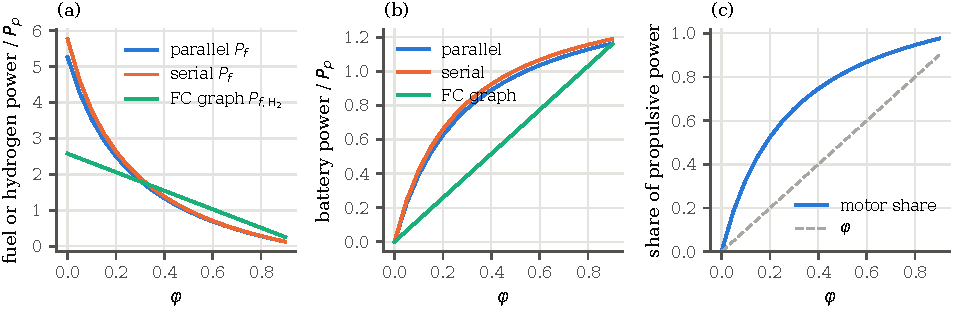
\includegraphics[width=\textwidth]{phi_sweep.pdf}
\caption{Graph solutions versus $\varphi$ at the reference efficiencies: (a) fuel or
hydrogen power, (b) battery terminal power, (c) share of $P_p$ delivered by the motor of the
parallel chain, $\eta_{gb}\eta_{pp}\Pi_2$.}\label{fig:phi}
\end{figure}

\subsection{Power ratios along the mission}
Figure~\ref{fig:mission} shows the powers and ratios at the 284 (parallel) and 283
(serial) accepted integration points of the design and diversion missions. The ratios come
from \code{Powertrain.Hybrid} at each point. Until the cruise, $\varphi = 0$ and the
parallel aircraft flies as a traditional one, with $\Pi_0 = 5.2609$. Along the cruise,
$\varphi$ ramps to 0.5, and $\Pi_0$ and $\Pi_5$ meet near 0.97 at the end of the ramp, as
Eq.~\eqref{eq:phi} requires. In the serial aircraft the motor shaft power equals the
propulsive power divided by $\eta_{gb}\eta_{pp}$ during the whole flight.

\begin{figure}[htbp]
\centering
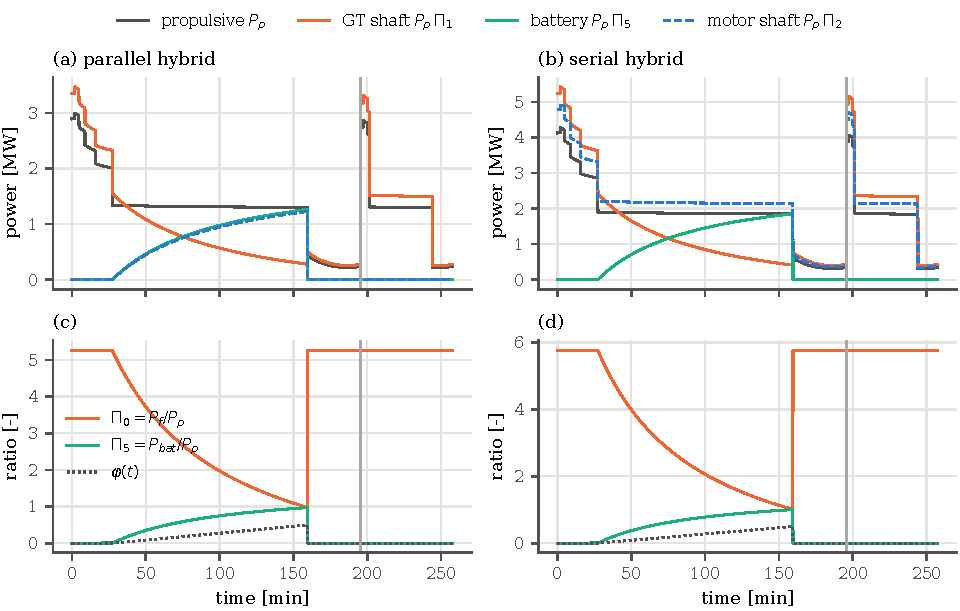
\includegraphics[width=\textwidth]{mission_ratios.pdf}
\caption{Parallel (left) and serial (right) Class-I reference designs: (a, b) propulsive,
gas-turbine shaft, battery and motor shaft powers; (c, d) fuel and battery ratios and
$\varphi(t)$. The vertical line marks the end of the design mission; the diversion
follows.}\label{fig:mission}
\end{figure}

\subsection{Powertrain mass}\label{sec:res-mass}
Table~\ref{tab:mass} and Figure~\ref{fig:mass} give the rating and the powertrain mass of
the six reference designs. In the three gas-turbine designs the engine rating is set by the
mission peak shaft power at \SI{1200}{m}, divided by $\lambda = 0.9161$. For instance, the
traditional peak of \SI{2846.5}{kW} gives \SI{3107.1}{kW}, above the take-off/OEI shaft
power of \SI{2675.2}{kW}; dividing by \SI{3900}{W/kg} gives \SI{796.7}{kg}.

\begin{table}[htbp]
\centering\small
\caption{Rating and powertrain mass of the reference designs. Masses in kg; the rating is
shaft power for the gas-turbine designs and SLS thrust for the turbofan.}\label{tab:mass}
\setlength{\tabcolsep}{3.5pt}
\begin{tabular}{@{}lrrrrrrr@{}}
\toprule
Design & $W_{TO}$ & Rating & Thermal & Generator & Motor & PMAD & $W_{PT}$ \\
\midrule
Traditional & 17\,843.1 & \SI{3107.1}{kW} & 796.7 & -- & -- & -- & 796.7 \\
Parallel & 21\,742.0 & \SI{3786.0}{kW} & 970.8 & -- & 252.7 & 126.3 & 1349.8 \\
Serial & 31\,034.3 & \SI{5921.3}{kW} & 1518.3 & 1184.3 & 989.9 & 515.6 & 4208.0 \\
Hydrogen & 21\,634.4 & -- & 1632.7$^a$ & -- & 381.6 & 385.5 & 2399.8 \\
FuelCellBattery & 40\,102.6 & -- & 3026.4$^a$ & -- & 707.4 & 714.5 & 4448.3 \\
Turbofan & 79\,883.5 & \SI{240.08}{kN} & 4449.6 & -- & -- & -- & 4449.6$^b$ \\
\bottomrule
\multicolumn{8}{@{}l}{\footnotesize $^a$ fuel-cell stack and balance of plant; the PMAD is
listed in its own column.}\\
\multicolumn{8}{@{}l}{\footnotesize $^b$ not added to the take-off-weight closure
(\code{avoid_powertrain_double_count}).}
\end{tabular}
\end{table}

\begin{figure}[htbp]
\centering
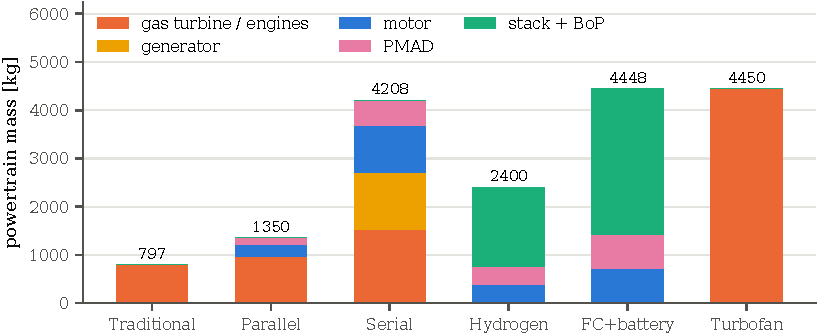
\includegraphics[width=0.95\textwidth]{mass_breakdown.pdf}
\caption{Powertrain mass breakdown of the reference designs (Table~\ref{tab:mass}). For the
fuel-cell designs, ``stack + BoP'' is the stack and balance of plant.}\label{fig:mass}
\end{figure}

The parallel motor and PMAD are sized on the battery peak of \SI{1263.4}{kW}; the take-off
battery power is zero because the take-off $\varphi$ is zero. The serial motor is sized on
its peak shaft power of \SI{4949.4}{kW}, the generator on the engine rating of
\SI{5921.3}{kW} and the PMAD on the bus peak of \SI{5155.6}{kW}. The serial electric drive
weighs \SI{2689.7}{kg}, against \SI{379.0}{kg} in the parallel design. Together with the
higher fuel ratio of the serial chain, this mass raises the take-off mass to
\SI{31034.3}{kg}. Without a battery (cruise $\varphi = 0$ throughout), the parallel design
closes at \SI{17842.7}{kg}, within \SI{0.4}{kg} of the traditional one; the two weight loops
use different Brent brackets (\num{1000}--\num{300000} and \num{10000}--\num{60000}~kg)
with the same tolerance of \SI{0.1}{kg}.

The fuel-cell drive follows Section~\ref{sec:mass-fc}. In the \code{'FuelCellBattery'}
design, \code{Max_PDrive} is \SI{5541.2}{kW}, equal to the peak of the fuel-cell propulsive
share: the peak falls where $\varphi = 0$, outside the cruise. The motor and the PMAD
(\SI{707.4}{kg} and \SI{714.5}{kg}) are therefore those of the fuel-cell share, on
\SI{7145.2}{kW} of electrical power.

The turbofan is sized by the mission peak: \SI{240.08}{kN} at sea level, against
\SI{198.74}{kN} for take-off/OEI and \SI{198.74}{kN} for the constraint diagram. The
nominal thrust at which the map is read is \SI{240.2}{kN}, so the required rating is
0.9995 times the nominal. This lies between the two thresholds of
\code{report_turbofan_sizing}, which therefore does not warn.

\subsection{Design sweep over the cruise \texorpdfstring{$\varphi$}{phi}}
Figure~\ref{fig:sweep} varies the end value of the linear cruise ramp of $\varphi$ from 0 to
0.5 for both hybrid topologies. Every design closes. The take-off mass of the parallel
design grows from \SI{17842.7}{kg} to \SI{21742.0}{kg} and that of the serial design from
\SI{25686.4}{kg} to \SI{31034.3}{kg}. The serial design is heavier at every $\varphi$
because its electric drive carries the full shaft power: \SI{2226.2}{kg} of motor, generator
and PMAD already at $\varphi = 0$. In both topologies the battery mass grows fastest, and the
gas turbine also grows, because the heavier aircraft needs more climb power.

\begin{figure}[htbp]
\centering
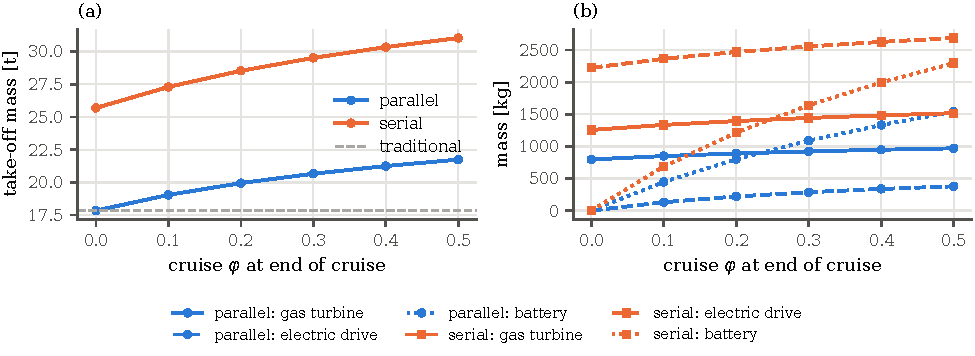
\includegraphics[width=\textwidth]{design_sweep.pdf}
\caption{Class-I hybrid designs versus the end value of the cruise $\varphi$ ramp: (a)
take-off mass, (b) gas-turbine, electric-drive and battery masses.}\label{fig:sweep}
\end{figure}

\subsection{Class-II motor in the parallel graph}\label{sec:res-motor}
Figure~\ref{fig:motor} uses the motor of example \code{05}: a d-q machine of
\SI{2000}{kW}, \SI{800}{V} and \SI{1200}{rpm}, evaluated at \SI{1200}{rpm}. Its efficiency is
0.970 at the design point and 0.968 at \SI{1}{MW}; it falls to 0.813 at \SI{0.1}{MW}.
Attached to the parallel graph at $\varphi = 0.3$, \SI{8000}{m} and \SI{120}{m/s}, it makes
$\Pi_5$ depend on the propulsive power: 0.9219 at $P_p = \SI{0.1}{MW}$ and 0.7859 at
\SI{3}{MW}, against 0.7802 with the constant $\eta_{em} = 0.98$. The model is read at the
motor shaft power $P_p\Pi_2$ (Section~\ref{sec:methods}), with $\Pi_2$ = 0.684 at
\SI{0.1}{MW} and 0.754 at \SI{3}{MW}. A \code{ConstantEfficiency(0.98)} assigned to
\code{em_model} reproduces the constant result exactly.

\begin{figure}[htbp]
\centering
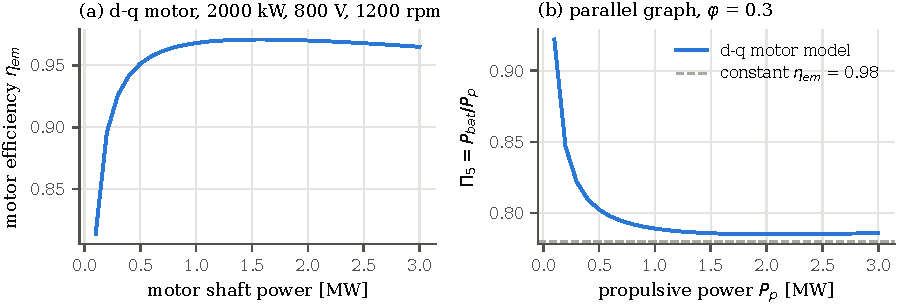
\includegraphics[width=0.95\textwidth]{motor_model.pdf}
\caption{(a) Efficiency of the d-q motor model versus its shaft power;
(b) the battery ratio of the parallel graph versus the propulsive power, with this model and
with the constant efficiency.}\label{fig:motor}
\end{figure}

\subsection{Turbofan node}
At the first accepted cruise point of the turbofan design (\SI{10058}{m},
\SI{233.4}{m/s}, $P_p$ = \SI{11.05}{MW}, thrust \SI{47.34}{kN}), the map gives
$\eta_o = 0.3231$ and \code{Powertrain.Traditional} returns
$[3.0950, 1, 1, 1]$. The product $\Pi_0\eta_o$ is 1.0, and the equivalent TSFC is
\SI{16.80}{g/(kN.s)} with $LHV$ = \SI{43}{MJ/kg}.

%% ======================================================================================
\section{Usage}\label{sec:usage}
%% ======================================================================================

The snippets run from \code{trunk/} with the package installed in the \code{phlygreen}
environment.

\subsection{Typed configuration}
The architecture is selected by two fields of \code{AircraftConfig}:
\code{configuration} and, for \code{'Hybrid'}, \code{hybrid_type}.
\code{AircraftConfig.__post_init__} rejects any other configuration name, a hybrid without
\code{'Parallel'} or \code{'Serial'}, and a turbofan with \code{weight_class='II'}. The
efficiencies and specific powers are fields of \code{EnergyConfig}.
\begin{lstlisting}
import sys; sys.path.insert(0, 'examples')
import PhlyGreen as pg
from common import hybrid_config

config = hybrid_config(battery_class='I', hybrid_type='Serial')
config.energy.specific_power_generator = 8000.0    # [W/kg]

aircraft = pg.build_aircraft()
aircraft.configure(config)                          # about 2 s

r = aircraft.results()
pt, m = aircraft.powertrain, aircraft.mission
print(r.WTO, r.WPT, r.engineRating, r.engineRating_units)
print(pt.WThermal, pt.WMotor, pt.WGenerator, pt.WPMAD)
print(m.Max_PEng, m.Max_PBat, m.Max_PMotor, m.Max_PBus)
\end{lstlisting}

\subsection{Legacy dictionaries}
The legacy API sets the flags on the aircraft and passes the efficiencies in
\code{EnergyInput} with the keys of Table~\ref{tab:inputs}:
\begin{lstlisting}
aircraft.Configuration = 'Hybrid'
aircraft.HybridType = 'Parallel'
EnergyInput = {'Ef': 43.5e6, 'Eta Gas Turbine': 0.22, 'Eta Gearbox': 0.96,
               'Eta Propulsive': 0.9, 'Eta PMAD': 0.99, 'Eta Electric Motor': 0.98,
               'Specific Power Powertrain': [3900, 5000], 'Specific Power PMAD': 10000}
\end{lstlisting}

\subsection{Evaluating the power balance}
A configured powertrain evaluates the power balance at any point, and a graph can be solved
on its own:
\begin{lstlisting}
pt = aircraft.powertrain
ratios = pt.Hybrid(0.3, 8000.0, 120.0, 1.0e6)   # phi, altitude [m], TAS [m/s], Pp [W]
fuel_power, battery_power = 1.0e6 * ratios[0], 1.0e6 * ratios[5]

from PhlyGreen.Systems.Powertrain.graph import parallel_hybrid_graph
sol = parallel_hybrid_graph(eta_gt=0.22, eta_gb=0.96, eta_pm=0.99,
                            eta_em=0.98, eta_pp=0.9, phi=0.3).solution()
print(sol['Pf'], sol['Pbat'])
\end{lstlisting}
\code{scripts/compute_data.py} calls \code{configure(config, design=False)} for this purpose:
it reads the inputs and builds the efficiencies without running the design.

\subsection{Attaching an efficiency model}
\begin{lstlisting}
from PhlyGreen.Systems.Powertrain.efficiency import (
    MotorEfficiencyModel, ResponseSurfaceEfficiency, make_efficiency_model)

pt.em_model = MotorEfficiencyModel(design_kw=2000, design_v=800, design_rpm=1200)
pt.em_model = make_efficiency_model(lambda op: 0.97 - 1.0e-9 * op.power)  # a law
pt.em_model = ResponseSurfaceEfficiency(lambda h, p: 0.95, ["altitude", "power"])
pt.em_model = None                                  # back to the constant Eta Electric Motor
\end{lstlisting}
An attribute set this way lives only on that aircraft object; \code{configure} builds a new
powertrain from the configuration. To size a design with the d-q motor, set
\code{config.energy.eta_electric_motor_model = 'Smart'} and \code{em_design_power},
as example \code{16_class_ii_propulsion_sizing.py} does.

\subsection{Reading the result}
Table~\ref{tab:outputs} lists where the design exposes the powertrain.

\begin{table}[htbp]
\centering\small
\caption{Powertrain outputs after a design.}\label{tab:outputs}
\begin{tabularx}{\textwidth}{@{}p{5.0cm}X@{}}
\toprule
Where & What \\
\midrule
\code{aircraft.results()} & \code{WPT} [kg], \code{engineRating} [W or N], \code{engineRating_units} (\code{'W'} or \code{'N'}) \\
\code{aircraft.weight.WPT} & powertrain mass; for the fuel-cell configurations the fuel-cell system mass \\
\code{aircraft.powertrain.WThermal} & gas-turbine or turbofan mass [kg] \\
\code{aircraft.powertrain.WMotor}, \code{WGenerator}, \code{WPMAD}, \code{WElectric} & electric-drive masses of a hybrid [kg]; \code{WMotor} includes \code{WGenerator} \\
\code{aircraft.powertrain.engineRating} & rating of Eq.~\eqref{eq:rating} [W], or $T_{rating}$ [N] \\
\code{aircraft.mission.Max_PEng}, \code{Max_PEng_alt}, \code{TO_PP} & peak shaft power, its altitude, take-off/OEI shaft power \\
\code{aircraft.mission.Max_PBat}, \code{TO_PBat} & battery terminal power peaks \\
\code{aircraft.mission.Max_PMotor}, \code{TO_PMotor}, \code{Max_PBus}, \code{TO_PBus} & motor shaft and motor input peaks \\
\code{aircraft.mission.Max_Thrust}, \code{TO_Thrust} & thrust peaks (every configuration) \\
\code{powertrain.report_turbofan_sizing()} & sizing case, required SLS thrust, the three cases, nominal ratio \\
\code{powertrain.report_class_ii_sizing()} & load ratios and status of the Class-II GT and motor \\
\code{PhlyGreen.postprocess.power_timeseries} & propulsive, gas-turbine and motor power along the mission \\
\bottomrule
\end{tabularx}
\end{table}

\subsection{Examples}
\begin{itemize}
\item \code{examples/01_design_traditional.py}, \code{02_hybrid_with_battery.py} and
  \code{02b_serial_hybrid.py} design the traditional, parallel and serial aircraft.
\item \code{examples/05_powertrain_graph_and_efficiency_models.py} solves a graph directly,
  attaches the d-q motor, builds the fuel-cell + battery graph and plots the Class-II maps.
\item \code{examples/15_class_i_vs_class_ii.py} and \code{16_class_ii_propulsion_sizing.py}
  use the Class-II gas turbine and motor with their nominal-power checks.
\item \code{examples/18_serial_range_extender_gt.py} flies the serial range extender.
\item \code{examples/23_fuelcell_battery_hybrid.py} and
  \code{25_fuelcell_battery_class_ii_models.py} cover the fuel-cell + battery aircraft.
\item \code{examples/26_turbofan_design.py} designs the turbofan.
\item \code{docs/user-guide/powertrain.md} and \code{docs/developer-guide/extending-the-model.md}
  are the user and developer guides.
\end{itemize}

\subsection{Pitfalls}
\begin{itemize}
\item \textbf{Meaning of $\varphi$.} In \code{'Hybrid'}, $\varphi$ is the battery share of
  the supplied power (Eq.~\eqref{eq:phi}). In \code{'FuelCellBattery'} it is the battery
  share of the propulsive power. The same profile gives different splits in the two
  configurations.
\item \textbf{Variable names.} In the serial graph $P_{gb}$ is the motor shaft power and
  $P_{gen}$ the gearbox output. Read the vectors by index (Table~\ref{tab:indices}).
\item \textbf{Silent defaults.} Without \texttt{Eta Gas Turbine} or \texttt{Eta Propulsive},
  \code{SetInput} prints a warning and the constant models use 0.30 and 0.85.
\item \textbf{Operating-point power.} A Class-II model receives the power of its own
  component, in the convention of Table~\ref{tab:convention}, for all engines together.
\item \textbf{Serial generator.} \code{em_model} and \code{'Smart'} act on the serial motor
  but not on the generator; replace \code{powertrain.efficiency['generator']} to make the
  generator operating-point dependent.
\item \textbf{Fuel-cell graph.} \code{PowerRatioFuelCellBattery} needs \texttt{Eta Fuel Cell}
  or an \code{fc_model} (Section~\ref{sec:fcb-graph}). Its battery entry is index 2.
\item \textbf{Turbofan rating.} \code{engineRating} is a thrust in newtons for
  \code{'Turbofan'}. Check \code{report_turbofan_sizing()} after the design: on the reference
  design the required thrust is 0.9995 times the nominal.
\end{itemize}

%% ======================================================================================
\section{Verification and limitations}\label{sec:verification}
%% ======================================================================================

\subsection{Tests}
The following tests cover the powertrain. We ran them on the code described here; all 104
tests in these eleven files passed.
\begin{itemize}
\item \code{tests/unit/test_powertrain_graph.py}: a lossless chain gives unit ratios; the
  traditional fuel ratio is the inverse of the efficiency product; a non-square system raises;
  an unknown variable raises; the split gives $P_{bat} = \varphi/(1-\varphi)\,P_f$ for four
  values of $\varphi$; the fuel-cell graph at $\varphi = 0$ inverts its chain and at
  $\varphi > 0$ uses the battery and less hydrogen; the serial graph is square and solvable.
\item \code{tests/unit/test_efficiency.py}: the constant, callable and response-surface models;
  \code{make_efficiency_model} for each kind of specification and its error; the d-q motor
  efficiency lies in range and depends on power; the motor mass is positive.
\item \code{tests/unit/test_turbofan_powertrain.py}: the turbofan graph is the traditional
  chain with unit gearbox and fan; $\eta_o$ and TSFC agree; the efficiency model converts
  power to thrust, rejects a standstill and requires a nominal thrust.
\item \code{tests/regression/test_powertrain_equivalence.py}: graph and legacy solvers agree
  (Section~\ref{sec:legacy}).
\item \code{tests/regression/test_class_ii_efficiency.py}: without a model the constant motor
  efficiency is used; a constant model reproduces it; the d-q motor makes the ratios depend on
  the operating point; \code{PowerRatioFuelCellBattery}; the gas-turbine map scales with size
  and lapses with altitude.
\item \code{tests/regression/test_sizing_denominator.py}: the sizing denominator equals the
  power lapse for power-rated configurations and leaves their design point unchanged.
\item \code{tests/regression/test_hybrid_bookkeeping.py}: among others, the serial motor and
  PMAD are sized on the shaft and bus powers.
\item \code{tests/regression/test_class_ii_sizing.py}: the nominal-power check of the Class-II
  gas turbine.
\item \code{tests/regression/test_turbofan.py}: the turbofan design, its sizing by the worst of
  three requirements and the TSFC/$\eta_o$ consistency on the sized aircraft.
\item \code{tests/regression/test_golden_design.py}: the traditional and parallel-hybrid
  golden masters.
\item \code{tests/regression/test_powertrain_component_powers.py}: each model is evaluated at
  the power through its own component in the four graphs; constant models are bit-identical
  to the plain graph; the serial motor uses the motor model; the fuel-cell graph $\varphi$ is
  the propulsive share and needs a fuel-cell efficiency; the engine count; the fuel-cell drive
  efficiencies; the range-extender flows.
\end{itemize}
The numbers of Section~\ref{sec:results} add three consistency checks. First, the graph and
legacy solvers agree to 0.0 on 198 points. Second, the parallel and serial vectors satisfy
Eqs.~\eqref{eq:par} and~\eqref{eq:ser}, and $\Pi_5/(\Pi_0 + \Pi_5) = \varphi$. Third, each
component mass equals its rated power over its specific power, for instance the serial motor
$\SI{4949.4}{kW}/\SI{5000}{W/kg} = \SI{989.9}{kg}$.

\subsection{Assumptions and limitations}
\begin{itemize}
\item \textbf{Steady power balance.} The graph is a steady, linear power balance with one
  efficiency per component. There are no power off-takes for the aircraft systems except the
  TMS pump of the fuel-cell configurations, no cable or bus losses beyond the PMAD
  efficiency, and no component dynamics.
\item \textbf{One split per graph.} The builders have one $\varphi$. A second degree of
  freedom needs a second split, as in Section~\ref{sec:new}.
\item \textbf{Operating point.} The Class-II models are evaluated at the power of their own
  component. In \code{'FuelCellBattery'} the two branches read the motor and propeller models
  at their own share of the power, not at the total power through the shared drive.
\item \textbf{Constant specific powers.} Every mass is a rating over a constant specific
  power. The gearbox has no mass of its own beyond what the thermal specific power covers.
  The default values (\SI{10000}{W/kg} for the PMAD, 5.5 for the engine thrust-to-weight) and
  the specific powers of \code{common.py} carry no source in the code.
\item \textbf{Parallel PMAD.} In the parallel hybrid the PMAD is sized on the battery power,
  not on the motor input power \code{Max_PBus} that the mission also tracks.
\item \textbf{Fuel-cell graph.} \code{fuelcell_battery_graph} is not used by any mission.
\item \textbf{Legacy equivalence.} The equivalence with the legacy solvers is established for
  constant efficiencies only.
\end{itemize}

%% ======================================================================================
\section{Input reference}\label{sec:inputs}
%% ======================================================================================

Table~\ref{tab:inputs} lists the inputs read by the powertrain. ``req.'' marks a key that
raises a \code{KeyError} when the configuration needs it and it is absent.
\code{EnergyConfig.__post_init__} checks that the efficiencies lie in $(0, 1]$ and that the
generator specific power is positive.

{\scriptsize
\setlength{\tabcolsep}{3pt}
\begin{longtable}{@{}>{\raggedright\arraybackslash}p{3.6cm}>{\raggedright\arraybackslash}p{3.7cm}>{\raggedright\arraybackslash}p{1.7cm}p{0.8cm}>{\raggedright\arraybackslash}p{4.6cm}@{}}
\caption{Powertrain inputs: \texttt{EnergyConfig} field (or other location), legacy key,
default, units and meaning.}\label{tab:inputs}\\
\toprule
Field & Legacy key & Default & Units & Meaning \\
\midrule
\endfirsthead
\toprule
Field & Legacy key & Default & Units & Meaning \\
\midrule
\endhead
\bottomrule
\endfoot
\multicolumn{5}{@{}l}{\emph{\code{AircraftConfig} (attributes of the \code{Aircraft})}}\\
\code{configuration} & \code{Configuration} & req. & -- & \code{'Traditional'}, \code{'Hybrid'}, \code{'Hydrogen'}, \code{'FuelCellBattery'}, \code{'Turbofan'} \\
\code{hybrid_type} & \code{HybridType} & req. (Hybrid) & -- & \code{'Parallel'} or \code{'Serial'} \\
\midrule
\multicolumn{5}{@{}l}{\emph{\code{EnergyConfig}: efficiencies}}\\
\code{eta_gas_turbine_model} & \texttt{Eta Gas Turbine Model} & \code{'constant'} & -- & \code{'constant'}, \code{'ResponseSurface'}, \code{'Turbofan'} \\
\code{eta_gas_turbine} & \texttt{Eta Gas Turbine} & 0.30 (warning) & -- & $\eta_{gt}$ \\
\code{eta_gearbox} & \texttt{Eta Gearbox} & req.; 1.0 for Turbofan & -- & $\eta_{gb}$ \\
\code{eta_propulsive_model} & \texttt{Eta Propulsive Model} & \code{'constant'} & -- & \code{'constant'}, \code{'Hamilton'}, \code{'Surrogate'}, \code{'RBF'} \\
\code{eta_propulsive} & \texttt{Eta Propulsive} & 0.85 (warning) & -- & $\eta_{pp}$ \\
\code{eta_pmad} & \texttt{Eta PMAD} & req. (Hybrid, fuel cell) & -- & $\eta_{pm}$ \\
\code{eta_electric_motor} & \texttt{Eta Electric Motor} & req. (Parallel, fuel cell) & -- & $\eta_{em}$ \\
\code{eta_electric_motor_1} & \texttt{Eta Electric Motor 1} & req. (Serial) & -- & generator, $\eta_{em1}$ \\
\code{eta_electric_motor_2} & \texttt{Eta Electric Motor 2} & req. (Serial) & -- & serial motor, $\eta_{em2}$ \\
\code{eta_fuel_cell} & \texttt{Eta Fuel Cell} & none (raises) & -- & $\eta_{fc}$ of \code{PowerRatioFuelCellBattery} only \\
\midrule
\multicolumn{5}{@{}l}{\emph{\code{EnergyConfig}: specific powers}}\\
\code{specific_power_powertrain} & \texttt{Specific Power Powertrain} & req.; [0, 0] for Turbofan & W/kg & [thermal $p_{th}$, motor $p_{em}$] \\
\code{specific_power_pmad} & \texttt{Specific Power PMAD} & 10000 & W/kg & $p_{PMAD}$ \\
\code{specific_power_generator} & \texttt{Specific Power Generator} & $p_{em}$ & W/kg & serial generator, $p_{gen}$ \\
\midrule
\multicolumn{5}{@{}l}{\emph{\code{EnergyConfig}: Class-II models and ratings}}\\
\code{eta_electric_motor_model} & \texttt{Eta Electric Motor Model} & constant & -- & \code{'Smart'} selects the d-q motor \\
\code{gt_design_power} & \texttt{GT Design Power} & \code{engineRating} & W & nominal gas-turbine shaft power (ResponseSurface) \\
\code{em_design_power} & \texttt{EM Design Power} & req. (Smart) & W & nominal motor power \\
\code{em_design_voltage} & \texttt{EM Design Voltage} & 800 & V & d-q motor voltage \\
\code{em_design_rpm} & \texttt{EM Design RPM} & 11000 & rpm & d-q motor speed \\
(none) & \texttt{Propeller RPM} & 1200 & rpm & propeller surrogate speed \\
\code{turbofan_design_thrust} & \texttt{Turbofan Design Thrust} & req. (Turbofan) & N & nominal SLS thrust, all engines \\
\code{engine_thrust_to_weight} & \texttt{Engine Thrust to Weight} & 5.5 & N/N & installed engine $(T/W)_{eng}$ \\
\code{turbofan_model_path} & \texttt{Turbofan Model Path} & packaged map & -- & alternative turbofan map \\
\midrule
\multicolumn{5}{@{}l}{\emph{\code{EnergyConfig}: serial range extender (Battery manual)}}\\
\code{gt_rated_power} & \texttt{GT Rated Power} & none & W & enables the range extender \\
\code{battery_charge_efficiency} & \texttt{Battery Charge Efficiency} & 1.0 & -- & in-flight recharge efficiency \\
\midrule
\multicolumn{5}{@{}l}{\emph{Other}}\\
(none) & \texttt{PropellerInput['Number of Engines']} & 2 & -- & \code{Powertrain.n_engines}: engines over which the Class-II models divide the power \\
\code{avoid_powertrain_double_count} & attribute of \code{Weight} & \code{False} & -- & see Section~\ref{sec:mass} \\
\end{longtable}
}

%% ======================================================================================
\section{Reproducing the figures}\label{sec:reproduce}
%% ======================================================================================

\begin{lstlisting}[language=bash]
python manuals/powertrain/scripts/compute_data.py    # phlygreen environment
python manuals/powertrain/scripts/make_figures.py
cd manuals/powertrain && latexmk -pdf -interaction=nonstopmode -outdir=build powertrain_manual.tex
\end{lstlisting}
\code{compute_data.py} runs the six reference designs and the 12 designs of the $\varphi$
sweep and writes \code{data/powertrain_data.json} in about \SI{85}{s}; the two fuel-cell
designs take \SI{26}{s} and \SI{31}{s}, the turbofan \SI{4}{s} and the others less than
\SI{2}{s} each.
\code{make_figures.py} reads the JSON file, writes the PDF plots and generates the TikZ
drawings \code{figures/graph_*.tex} from the graph builders in about \SI{3}{s}. With
\code{--recompute} it runs \code{compute_data.py} first.

%% ======================================================================================
\begin{thebibliography}{9}\small
\bibitem{devries2019} R.~de~Vries, M.~Brown and R.~Vos. Preliminary sizing method for
  hybrid-electric distributed-propulsion aircraft. \emph{Journal of Aircraft},
  56(6):2172--2188, 2019. Cited in the class docstring of \code{Powertrain}.
\bibitem{ruijgrok} Ruijgrok. \emph{Elements of Airplane Performance}, Eq.~(6.7-11). Cited in
  the docstring of \code{Powertrain.PowerLapse}.
\end{thebibliography}

\end{document}
